\documentclass[12pt,twoside]{article}

\newcommand{\reporttitle}{Deep Learning For Facial Expression Analysis}
\newcommand{\reportauthor}{Tom Bartissol}
\newcommand{\reporttype}{Final Report}
\newcommand{\cid}{00824562}

% paragraph skip length
\setlength{\parskip}{1em}
% line spacing
\renewcommand{\baselinestretch}{1.3}
\newcommand{\source}[1]{\vspace{-3pt} \caption*{ \footnotesize{\textit{Source: {#1}}}} }
\setcounter{secnumdepth}{6}
\newcommand{\para}[1]{\paragraph{#1}\mbox{}\\}


% include files that load packages and define macros
%%%%%%%%%%%%%%%%%%%%%%%%%%%%%%%%%%%%%%%%%
% University Assignment Title Page 
% LaTeX Template
% Version 1.0 (27/12/12)
%
% This template has been downloaded from:
% http://www.LaTeXTemplates.com
%
% Original author:
% WikiBooks (http://en.wikibooks.org/wiki/LaTeX/Title_Creation)
%
% License:
% CC BY-NC-SA 3.0 (http://creativecommons.org/licenses/by-nc-sa/3.0/)
% 
% Instructions for using this template:
% This title page is capable of being compiled as is. This is not useful for 
% including it in another document. To do this, you have two options: 
%
% 1) Copy/paste everything between \begin{document} and \end{document} 
% starting at \begin{titlepage} and paste this into another LaTeX file where you 
% want your title page.
% OR
% 2) Remove everything outside the \begin{titlepage} and \end{titlepage} and 
% move this file to the same directory as the LaTeX file you wish to add it to. 
% Then add \input{./title_page_1.tex} to your LaTeX file where you want your
% title page.
%
%----------------------------------------------------------------------------------------
%	PACKAGES AND OTHER DOCUMENT CONFIGURATIONS
%----------------------------------------------------------------------------------------
\usepackage{ifxetex}
\usepackage{textpos}
\usepackage{natbib}
\usepackage{kpfonts}
\usepackage[a4paper,hmargin=2.8cm,vmargin=2.0cm,includeheadfoot]{geometry}
\usepackage{ifxetex}
\usepackage{stackengine}
\usepackage{tabularx,longtable,multirow,caption}%hangcaption
\usepackage{fncylab} %formatting of labels
\usepackage{fancyhdr}
\usepackage{color}
\usepackage[tight,ugly]{units}
\usepackage{url}
\usepackage{float}
\usepackage[english]{babel}
\usepackage{amsmath}
\usepackage{graphicx}
\usepackage[colorinlistoftodos]{todonotes}
\usepackage{dsfont}
\usepackage{epstopdf} % automatically replace .eps with .pdf in graphics
\usepackage{natbib}
\usepackage{backref}
\usepackage{array}
\usepackage{latexsym}
\usepackage{etoolbox}

\usepackage{enumerate} % for numbering with [a)] format 



\ifxetex
\usepackage{fontspec}
\setmainfont[Scale=.8]{OpenDyslexic-Regular}
\else
\usepackage[pagebackref,hypertexnames=false,colorlinks]{hyperref} % provide links in pdf
\hypersetup{pdftitle={},
  pdfsubject={}, 
  pdfauthor={\reportauthor},
  pdfkeywords={}, 
  pdfstartview=FitH,
  pdfpagemode={UseOutlines},% None, FullScreen, UseOutlines
  bookmarksnumbered=true, bookmarksopen=true, colorlinks,
    citecolor=green,%
    filecolor=black,%
    linkcolor=black,%
    urlcolor=black}
\usepackage[all]{hypcap}
\fi

\usepackage{tcolorbox}

% various theorems
\usepackage{ntheorem}
\theoremstyle{break}
\newtheorem{lemma}{Lemma}
\newtheorem{theorem}{Theorem}
\newtheorem{remark}{Remark}
\newtheorem{definition}{Definition}
\newtheorem{proof}{Proof}

% example-environment
\newenvironment{example}[1][]
{ 
\vspace{4mm}
\noindent\makebox[\linewidth]{\rule{\hsize}{1.5pt}}
\textbf{Example #1}\\
}
{ 
\noindent\newline\makebox[\linewidth]{\rule{\hsize}{1.0pt}}
}



%\renewcommand{\rmdefault}{pplx} % Palatino
% \renewcommand{\rmdefault}{put} % Utopia

\ifxetex
\else
\renewcommand*{\rmdefault}{bch} % Charter
\renewcommand*{\ttdefault}{cmtt} % Computer Modern Typewriter
%\renewcommand*{\rmdefault}{phv} % Helvetica
%\renewcommand*{\rmdefault}{iwona} % Avant Garde
\fi

\setlength{\parindent}{4em}  % indentation of paragraph

\setlength{\headheight}{14.5pt}
\pagestyle{fancy}
\fancyfoot[ER,OL]{\thepage}%Page no. in the left on
                                %odd pages and on right on even pages
\fancyfoot[OC,EC]{\sffamily }
\renewcommand{\headrulewidth}{0.1pt}
\renewcommand{\footrulewidth}{0.1pt}
\captionsetup{margin=10pt,font=small,labelfont=bf}


%--- chapter heading

\def\@makechapterhead#1{%
  \vspace*{10\p@}%
  {\parindent \z@ \raggedright %\sffamily
        %{\Large \MakeUppercase{\@chapapp} \space \thechapter}
        %\\
        %\hrulefill
        %\par\nobreak
        %\vskip 10\p@
    \interlinepenalty\@M
    \Huge \bfseries 
    \thechapter \space\space #1\par\nobreak
    \vskip 30\p@
  }}

%---chapter heading for \chapter*  
\def\@makeschapterhead#1{%
  \vspace*{10\p@}%
  {\parindent \z@ \raggedright
    \sffamily
    \interlinepenalty\@M
    \Huge \bfseries  
    #1\par\nobreak
    \vskip 30\p@
  }}
  



% %%%%%%%%%%%%% boxit
\def\Beginboxit
   {\par
    \vbox\bgroup
	   \hrule
	   \hbox\bgroup
		  \vrule \kern1.2pt %
		  \vbox\bgroup\kern1.2pt
   }

\def\Endboxit{%
			      \kern1.2pt
		       \egroup
		  \kern1.2pt\vrule
		\egroup
	   \hrule
	 \egroup
   }	

\newenvironment{boxit}{\Beginboxit}{\Endboxit}
\newenvironment{boxit*}{\Beginboxit\hbox to\hsize{}}{\Endboxit}



\allowdisplaybreaks

\makeatletter
\newcounter{elimination@steps}
\newcolumntype{R}[1]{>{\raggedleft\arraybackslash$}p{#1}<{$}}
\def\elimination@num@rights{}
\def\elimination@num@variables{}
\def\elimination@col@width{}
\newenvironment{elimination}[4][0]
{
    \setcounter{elimination@steps}{0}
    \def\elimination@num@rights{#1}
    \def\elimination@num@variables{#2}
    \def\elimination@col@width{#3}
    \renewcommand{\arraystretch}{#4}
    \start@align\@ne\st@rredtrue\m@ne
}
{
    \endalign
    \ignorespacesafterend
}
\newcommand{\eliminationstep}[2]
{
    \ifnum\value{elimination@steps}>0\leadsto\quad\fi
    \left[
        \ifnum\elimination@num@rights>0
            \begin{array}
            {@{}*{\elimination@num@variables}{R{\elimination@col@width}}
            |@{}*{\elimination@num@rights}{R{\elimination@col@width}}}
        \else
            \begin{array}
            {@{}*{\elimination@num@variables}{R{\elimination@col@width}}}
        \fi
            #1
        \end{array}
    \right]
    & 
    \begin{array}{l}
        #2
    \end{array}
    &%                                    moved second & here
    \addtocounter{elimination@steps}{1}
}
\makeatother

%% Fast macro for column vectors
\makeatletter  
\def\colvec#1{\expandafter\colvec@i#1,,,,,,,,,\@nil}
\def\colvec@i#1,#2,#3,#4,#5,#6,#7,#8,#9\@nil{% 
  \ifx$#2$ \begin{bmatrix}#1\end{bmatrix} \else
    \ifx$#3$ \begin{bmatrix}#1\\#2\end{bmatrix} \else
      \ifx$#4$ \begin{bmatrix}#1\\#2\\#3\end{bmatrix}\else
        \ifx$#5$ \begin{bmatrix}#1\\#2\\#3\\#4\end{bmatrix}\else
          \ifx$#6$ \begin{bmatrix}#1\\#2\\#3\\#4\\#5\end{bmatrix}\else
            \ifx$#7$ \begin{bmatrix}#1\\#2\\#3\\#4\\#5\\#6\end{bmatrix}\else
              \ifx$#8$ \begin{bmatrix}#1\\#2\\#3\\#4\\#5\\#6\\#7\end{bmatrix}\else
                 \PackageError{Column Vector}{The vector you tried to write is too big, use bmatrix instead}{Try using the bmatrix environment}
              \fi
            \fi
          \fi
        \fi
      \fi
    \fi
  \fi 
}  
\makeatother

\robustify{\colvec}

%%% Local Variables: 
%%% mode: latex
%%% TeX-master: "notes"
%%% End: 
 % various packages needed for maths etc.
% quick way of adding a figure
\newcommand{\fig}[3]{
 \begin{center}
 \scalebox{#3}{\includegraphics[#2]{#1}}
 \end{center}
}

%\newcommand*{\point}[1]{\vec{\mkern0mu#1}}
\newcommand{\ci}[0]{\perp\!\!\!\!\!\perp} % conditional independence
\newcommand{\point}[1]{{#1}} % points 
\renewcommand{\vec}[1]{{\boldsymbol{{#1}}}} % vector
\newcommand{\mat}[1]{{\boldsymbol{{#1}}}} % matrix
\newcommand{\R}[0]{\mathds{R}} % real numbers
\newcommand{\Z}[0]{\mathds{Z}} % integers
\newcommand{\N}[0]{\mathds{N}} % natural numbers
\newcommand{\nat}[0]{\mathds{N}} % natural numbers
\newcommand{\Q}[0]{\mathds{Q}} % rational numbers
\ifxetex
\newcommand{\C}[0]{\mathds{C}} % complex numbers
\else
\newcommand{\C}[0]{\mathds{C}} % complex numbers
\fi
\newcommand{\tr}[0]{\text{tr}} % trace
\renewcommand{\d}[0]{\mathrm{d}} % total derivative
\newcommand{\inv}{^{-1}} % inverse
\newcommand{\id}{\mathrm{id}} % identity mapping
\renewcommand{\dim}{\mathrm{dim}} % dimension
\newcommand{\rank}[0]{\mathrm{rk}} % rank
\newcommand{\determ}[1]{\mathrm{det}(#1)} % determinant
\newcommand{\scp}[2]{\langle #1 , #2 \rangle}
\newcommand{\kernel}[0]{\mathrm{ker}} % kernel/nullspace
\newcommand{\img}[0]{\mathrm{Im}} % image
\newcommand{\idx}[1]{{(#1)}}
\DeclareMathOperator*{\diag}{diag}
\newcommand{\E}{\mathds{E}} % expectation
\newcommand{\var}{\mathds{V}} % variance
\newcommand{\gauss}[2]{\mathcal{N}\big(#1,\,#2\big)} % gaussian distribution N(.,.)
\newcommand{\gaussx}[3]{\mathcal{N}\big(#1\,|\,#2,\,#3\big)} % gaussian distribution N(.|.,.)
\newcommand{\gaussBig}[2]{\mathcal{N}\left(#1,\,#2\right)} % see above, but with brackets that adjust to the height of the arguments
\newcommand{\gaussxBig}[3]{\mathcal{N}\left(#1\,|\,#2,\,#3\right)} % see above, but with brackets that adjust to the height of the arguments
\DeclareMathOperator{\cov}{Cov} % covariance (matrix) 
\ifxetex
\renewcommand{\T}[0]{^\top} % transpose
\else
\newcommand{\T}[0]{^\top}
\fi
% matrix determinant
\newcommand{\matdet}[1]{
\left|
\begin{matrix}
#1
\end{matrix}
\right|
}



%%% various color definitions
\definecolor{darkgreen}{rgb}{0,0.6,0}

\newcommand{\blue}[1]{{\color{blue}#1}}
\newcommand{\red}[1]{{\color{red}#1}}
\newcommand{\green}[1]{{\color{darkgreen}#1}}
\newcommand{\orange}[1]{{\color{orange}#1}}
\newcommand{\magenta}[1]{{\color{magenta}#1}}
\newcommand{\cyan}[1]{{\color{cyan}#1}}


% redefine emph
\renewcommand{\emph}[1]{\blue{\bf{#1}}}

% place a colored box around a character
\gdef\colchar#1#2{%
  \tikz[baseline]{%
  \node[anchor=base,inner sep=2pt,outer sep=0pt,fill = #2!20] {#1};
    }%
}%
 % short-hand notation and macros

\usepackage{bm}
\usepackage[toc,page]{appendix}
\usepackage{slashbox}
\usepackage{subcaption}

\newcommand{\ackname}{Acknowledgements}

%%%%%%%%%%%%%%%%%%%%%%%%%%%%

\begin{document}
% front page
% Last modification: 2016-09-29 (Marc Deisenroth)
\begin{titlepage}

\newcommand{\HRule}{\rule{\linewidth}{0.5mm}} % Defines a new command for the horizontal lines, change thickness here


%----------------------------------------------------------------------------------------
%	LOGO SECTION
%----------------------------------------------------------------------------------------


\includegraphics[width = 4cm]{./figures/imperial.eps}\\[0.5cm] 

\begin{center} % Center remainder of the page

%----------------------------------------------------------------------------------------
%	HEADING SECTIONS
%----------------------------------------------------------------------------------------
\textsc{\LARGE \reporttype}\\[1.5cm] 
\textsc{\Large Imperial College London}\\[0.5cm] 
\textsc{\large Department of Computing}\\[0.5cm] 
%----------------------------------------------------------------------------------------
%	TITLE SECTION
%----------------------------------------------------------------------------------------

\HRule \\[0.4cm]
{ \huge \bfseries \reporttitle}\\ % Title of your document
\HRule \\[1.5cm]
\end{center}
%----------------------------------------------------------------------------------------
%	AUTHOR SECTION
%----------------------------------------------------------------------------------------

%\begin{minipage}{0.4\hsize}
\begin{flushleft} \large
\textit{Author:}\\
\reportauthor~(CID: \cid) % Your name
\end{flushleft}
\vspace{2cm}
\makeatletter
Date: \@date 

\vfill % Fill the rest of the page with whitespace



\makeatother


\end{titlepage}



%%%%%%%%%%%%%%%%%%%%%%%%%%%% ABSTRACT
\cleardoublepage
\begin{abstract}
  Humans can communicate through multiple channels including speech and facial
  expressions. Enabling machines to understand these channels would unlock a
  multitude of opportunities for Human Computer Interaction and while progress
  has been made on the speech side, facial expressions remain more complex for a
  machine to understand.

  However, with the advent of Deep Learning models in recent years, this goal might be within
  reach. We use two such models, Inception V2 and VGG 16, to classify Action Units with a maximal
  accuracy of 88.9\% on a subset of EmotioNet and to predict Valence and
  Arousal of facial expressions with a best root mean squared error of 3.71.
\end{abstract}
\cleardoublepage

\thispagestyle{empty}
\section*{\ackname}

I would like to thank the following people for their contributions to this
project:

\begin{itemize}
  \item my project supervisor, Stefanos Zafeiriou
  \item PhD student Dimitris Kollias for taking the time to patiently answer my
    questions
  \item my friends and family for their continuous and unconditional support
\end{itemize}

\cleardoublepage
\tableofcontents
\clearpage
%%%%%%%%%%%%%%%%%%%%%%%%%%%% Main document



\section{Introduction}

The ability to analyse human facial expressions is an active area of research
with exciting near-future real-world applications ranging from law enforcement
to advertising (measuring how positively or negatively people respond to an
ad). It would also be at the core of any system capable of intelligent
Human-Computer Interaction (HCI). Indeed, for such interactions to be
life-like, the Computer should be able to recognise human emotions which are
expressed through multiple channels, an important one being facial expressions.
\textit{Interpreting} the recognised facial expressions into the six
\textit{basic emotions} \cite{RefWorks:12} (see Table ~\ref{tab:emo-au}), 
or better yet, on two continuous emotion dimensions,
would allow the Computer to identify human emotions to some extent.

Facial Expressions result from the contraction of a facial muscle or a group of facial muscles and the visually perceptible changes due to such contractions have been codified by Ekman and Friesen into the well-known Facial Action Coding System (FACS) \cite{RefWorks:10} which provides labels, facial \textit{Action Units} (AUs), for the actions of a muscle or group of muscles. For instance, AU 12 corresponds the lip corner puller and if it is active at the same time as AU 6, which corresponds to the cheek raiser, then the subject is smiling and this could be interpreted as happiness.

We are therefore concerned with two problems (i) identifying whether these AUs
are active or not and (ii) estimating continuous emotion dimensions: valence 
(how positive or negative the emotion is) and arousal (how intense) instead of 
discrete emotions such as the six basic emotions. We are therefore interested
in images of facial expressions. More specifically, whereas the majority of previous 
work has been conducted on data sets captured in constrained environment and/or using 
acted or posed facial expressions \cite{RefWorks:2}, we are interested in the so 
called "\textit{in-the-wild}" images, which are taken in different lighting conditions 
with different poses and most accurately represent spontaneous facial expressions.

To achieve this, we will use end-to-end deep learning models, namely VGG 16 and
Inception V2. Each model will be fine-tuned to solve problems (i) and (ii) on
data taken in-the-wild, and more precisely on the EmotioNet \cite{RefWorks:1} database 
Finally we will evaluate these models on an independent subset of the same
database.

\clearpage
\section{Background}

\subsection{Facial Expressions}

\subsubsection{Facial Action Coding System (FACS)}

The human head having a finite number of muscles, the number of visually
perceptible changes that can be caused by the contraction or relaxation of one
or more of these muscles, that is the number of facial expressions, is finite.
We can therefore taxonomise these facial changes into a coding system. Although
there exists a few such coding systems \cite{RefWorks:13}, the most popular and
used coding system is the FACS \cite{RefWorks:10}. FACS breaks down each
\textit{visually perceptible} change into facial \textit{Action Units} (AUs) which roughly corresponds to the contraction or relaxation of individual facial muscles. The activation of one or more AU creates a facial expression. Some examples of AUs and their associated facial are listed in Figure ~\ref{fig:fau}.

On top of this taxonomy, FACS also provides an intensity score, A-E
(maximum-minimum), to rate how \textit{pronounced} each AU is in a facial expression (see Table ~\ref{tab:scale-au}). For instance AU 12A would indicate that the lip corners are slightly pulled whereas AU 12E would indicate that they are maximally pulled.

Finally, AUs do not activate instantly. Indeed, an AU is firstly in a neutral
state, then, when it starts activating, muscles contract and the AU is said to
be in an \textit{onset} phase, once the muscles are contracted and the AU is at
its peak, it is said to be in an \textit{apex} phase, finally, when the muscles
start to relax and the AU starts to disappear, the AU is said to be in an
\textit{offset} phase before returning to normal. So the activation of an AU
generally follows the following pattern: neutral - onset - apex - offset -
neutral, see Fig.~\ref{fig:onset}.

\begin{table}[ht]
\centering
\begin{tabular}{|l|l|}
 \hline
 Intensity & description\\
 \hline
 \hline
 A & Trace                \\
 \hline
 B & Slight               \\
 \hline
 C & Marked or Pronounced \\
 \hline
 D & Severe or Extreme    \\
 \hline
 E & Maximal              \\
 \hline
\end{tabular}
\caption{The scale for measuring the intensity with which an AU is activated}
\label{tab:scale-au}
\end{table}

\begin{figure}
\centering
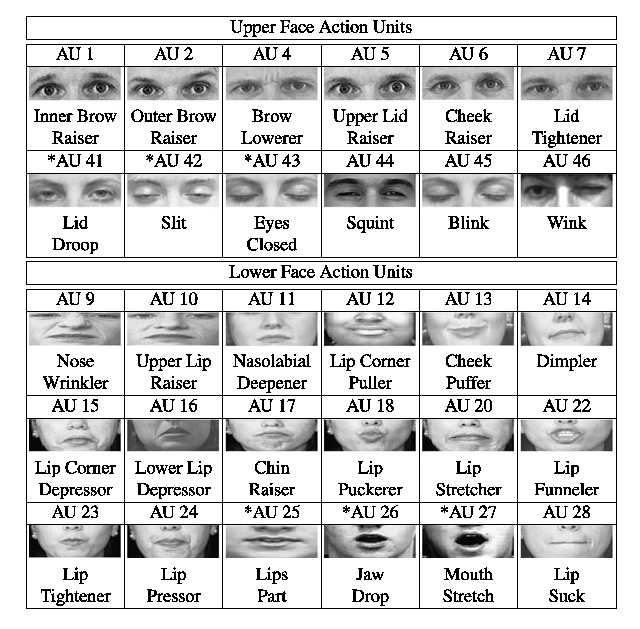
\includegraphics[scale=1]{./figures/faus.eps}
\caption{Facial Action Units}
\label{fig:fau}
\end{figure}

\begin{figure}[ht]
  \centering
  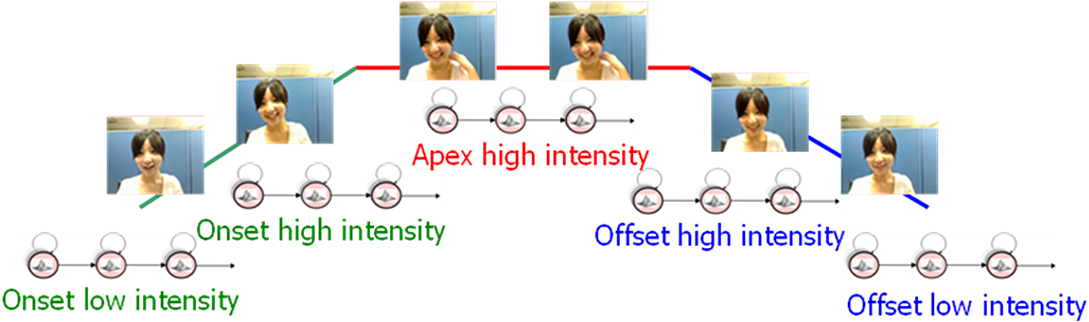
\includegraphics[width=1\textwidth]{figures/onset.jpg}
  \caption{The neutral-onset-apex-offset-neutral cycle of an action unit
  activation}
  \source{http://proj.ncku.edu.tw/research/articles/e/20150508/images/150427015117V6MKPn.jpg}
  \label{fig:onset}
\end{figure}

\subsubsection{Interpreting emotions}

\para{Discrete case}
Emotions can roughly be broken down into six \textit{basic emotions} \cite{RefWorks:12}, 
seven if we count the neutral emotion. We can then interpret a facial expression into 
one of these seven categories. Note that this is only an interpretation as emotions 
are expressed through multiple channels such as body language or voice and facial 
expressions are only one of these channels.


\para{Continuous case}
This is the case in which we are interested. Emotions can be represented using two continuous dimensions:

\begin{itemize}
\item \textbf{Valence}: characterises the attractiveness or aversivenes of an emotion, that is respectfully how positive or negative the emotion is.
\item \textbf{Arousal}: characterises the intensity of the emotion, as such high
  arousal would indicate a state of increased activity and alertness of mind and body
  (e.g. fear or excitement).
\end{itemize}

We can therefore represent emotions in a two dimensional coordinate system using their valence and arousal values, see Figure ~\ref{fig:arval} 

\begin{figure}[h]
\centering
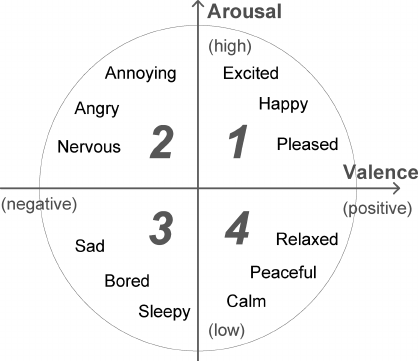
\includegraphics[scale=0.6]{./figures/valence_arousal_plot.png}
\caption{Plotting emotions according to their valence and arousal}
\source{https://www.researchgate.net/profile/Yi-hsuan\_Yang/publication/254004106}
\label{fig:arval}
\end{figure}

\begin{table}[h]
\centering
\begin{tabular}{|l|l|}
 \hline
 Emotion & AUs\\
 \hline
 \hline
 Neutral   & 0                     \\
 \hline
 Happiness & 6, 12                 \\
 \hline
 Sadness   & 1, 4, 14              \\
 \hline
 Surprise  & 1, 2, 5B, 26          \\
 \hline
 Fear      & 1, 2, 4, 5, 7, 20, 26 \\
 \hline
 Anger     & 4, 5, 7, 23           \\
 \hline
 Disgust   & 9, 15, 16             \\
 \hline
\end{tabular}
\caption{The 6 basic emotions (plus neutral) and the corresponding Action Units that are generally activate when the emotion is present}
\label{tab:emo-au}
\end{table}

%%%%% EARLY DAYS %%%%%
\subsection{Facial Expression Analysis}

In the early days, facial expression analysis was restricted to recognising the six basic emotions. Furthermore, computer vision techniques were used to extract features from input images and then classify them instead of using the \textit{end-to-end} deep learning techniques we will use in this project. As indicated in \cite{RefWorks:2}, the interested reader is directed towards \cite{RefWorks:18,RefWorks:19} for a thorough overview of these early techniques.

\subsection{Database - EmotioNet}\label{sec:databases}

We direct the reader towards \cite{RefWorks:2} for a complete survey of the
main databases available for facial expression analysis. We are interested in
databases containing images or videos taken in-the-wild and annotated with
facial action units. As such, we will use the EmotioNet \cite{RefWorks:1}
database which contains 1,000,000 in-the-wild images of emotions. These images
were downloaded from the Internet by using specific combinations of keywords,
such as ``feeling angry'' or ``feeling happy'',
and were then automatically annotated with AUs and AU intensities as well as
emotion categories by using a novel computer vision algorithm presented in
\cite{RefWorks:1}.

However, we are interested in a subset of 25,000 images from this database that
were manually annotated as we consider the accuracy of these annotations to be
higher than those produced by the algorithm mentioned above. This subset was
annotated for Action Units activation with '1' meaning that the action unit is
active, '0' that is not active and '999' that the action unit is occluded or
that it has not been annotated. An example image from this dataset is
presented in Fig.~\ref{fig:emotionet_example}

\begin{figure}[ht]
  \centering
  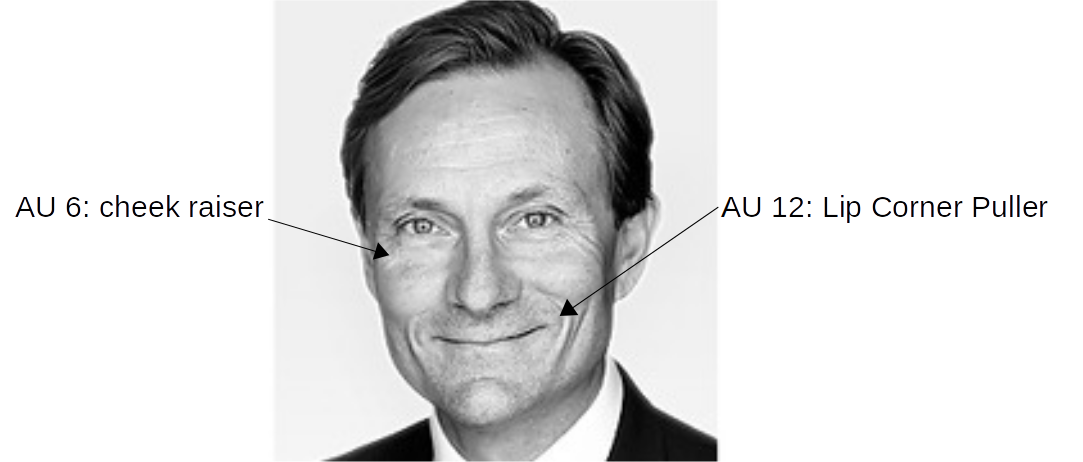
\includegraphics[scale=0.7]{./figures/emotionet_example.png}
  \caption{Example image from the EmotioNet database. Only two AUs, 6 and 12,
  are labelled as active (i.e. '1'). AUs 1, 2, 4, 5, 9, 17, 20, 25, and 26
are labelled as inactive and the remaining AUs are labelled as occluded or '999'}
  \label{fig:emotionet_example}
\end{figure}



\subsection{Deep Learning}

We use deep learning models in order to, given an image of a facial expression,
recognise which AUs are active and which aren't as well as estimate the valence and
arousal of the given facial expression. We use these models as they have proved
to be able to learn to represent abstract data features (e.g a smile) by using
multiple computational layers.

More formally, a deep learning model is a neural network with a set of
$n$ layers. Let $a_j^i$ be the output, or activation, of the $j^{th}$ neuron of
the $i^{th}$ layer for $i = 1 \dots n$ where the case $i=1$ corresponds to the
input vector. Then we can relate $a_j^i$ to the outputs of the previous layer
as follows:

\begin{align}
  a_j^i &= f\left( z_j^i  \right)\\
  z_j^i &= s_j^i + b_j^i 
  \label{eq:NN}
\end{align}

Where $s_j^i$ is the some weighted sum of all or part of the activations
$a_j^{i-1}$ for $j = 1 \dots m_{i-1}$ (where $m_{i-1}$ is the number of
neurons in layer $i-1$) of the previous layer, $b_j^i$ is a \textit{bias term} and
$f(.)$ is an \textit{activation function} which ensures non linearity.

\subsubsection{Deep Convolutional Neural Networks}

In particular, since our task focuses on images (i.e. 2/3-dimensional data), we
will be using a particular type of deep learning models called Deep
Convolutional Neural Networks (DCNNs). DCNNs consist of a succession of 
convolutional and pooling layers followed by fully connected layers.

\begin{figure}[ht]
  \centering
  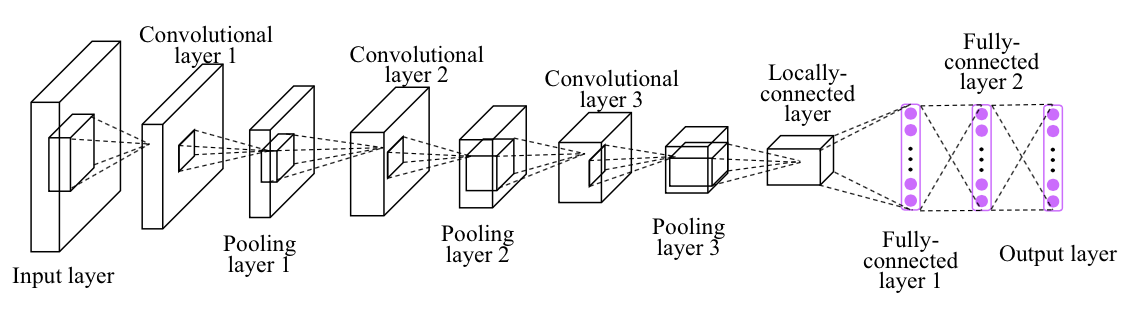
\includegraphics[scale=0.8]{figures/cnn.png}
  \caption{example of a DCNN architecture with a succession of convolutional +
  max pooling layers followed by a bloc of fully connected layers}
  \source{http://personal.ie.cuhk.edu.hk/~ccloy/project\_target\_code/images/fig3.png}
  \label{fig:cnn}
\end{figure}

The first block of layers, the convolutional and pooling layers, act as a feature
extractor. They take as input a raster image $\in \mathcal{R}^{nxm}$ where 
$n$ is the image height and $m$ the image width, either in greyscale ($\in
\mathcal{R}^{1xnxm}$) or in RGB colours $\in \mathcal{R}^{3xnxm}$ 
(where 3 is the depth of the image, i.e. the number of channels) and
processes it to extract features which will constitute a meaningful
representation of the image in a lower dimension, i.e. a vector.

\para{Convolutional Layers}

Convolutional layers are the core components of DCNNs. They are were the most
heavy computations take place and act as feature extractors by applying a set
of spatially small learnable kernel filters to the input image. 
These filters could  for instance have a
size of 7x7x$D$ where the first and the second 7 correspond to the height and the
width of the filter respectively and $D$ corresponds to the depth (e.g. 1 for
greyscale or 3 if we are working with RGB input images).

Each filter is applied by ``sliding'' it over the input image and performing a
convolution at every pixel of the image between the filter and the portion of 
the image that lies directly beneath it. Mathematically, this gives the
following: suppose we have an input image $I \in \mathcal{R}^{WxH}$ and a
filter $F \in \mathcal{R}^{kxk}$ such that $I(a,b)$ denotes the pixel on row
$a$ and column $b$ of $I$ (assume the same notation for $F$). Then the convolution
operation  $C(\cdot,\cdot)$ executed at pixel $(a,b)$ of the image is

\begin{equation}
  C(a,b) = \sum_{i=1}^{k}\sum_{j=1}^{k} F(i,j) \times I(a-i, b-j)
  \label{eq:convolution}
\end{equation}

Therefore, as we slide a filter over the image, we produce a 2D response map
that corresponds to the convolved features at each spatial location of the
input image, see Fig.~\ref{fig:conv_op}. Intuitively, each kernel filter learns
to detect specific features in the input space such as as corner or a blob of colour

In the case of a 3 dimensional input volume ($Width \times Height \times Depth$), each filter will also be 3
dimensional with the depth dimension $D$ matching that of the input. Therefore each
filter will produce $D$ response maps which are summed together with a bias
term to produce a 2 dimensional overall response map for that filter.

Finally, when using a $k\times k$ kernel on an $n \times m$ image, the response map will have a smaller
size of $(n-l)\times(m-l)$ where $l=\frac{k-1}{2}$ ($k$ is and odd
number). While we do want to perform dimensionality reduction before going
through the fully connected layers, this means that the kernel might omit some
important features that are at the edges of the image. To solve this problem,
it is common practice to add $l$ layers of \textit{zero-padding} on each side of the
image so that the kernel also covers the edges of the image and the response
map has the same dimension as the input.

To sum up, here are the inputs and the outputs of a typical convolutional
layer with $N$ kernel features of size $k \times k$ applied using a stride of
$s$ on an image with a padding of $p$:

\begin{enumerate}
  \item \textbf{In}: an image with size $W \times H \times D$ where $W$ is the
    width of the image, $H$ the height and $D$ the depth
  \item \textbf{Out}: a volume with size $W_{out} \times H_{out} \times N$
    where $W_{out} = \frac{W - k + 2p}{s}$, $H_{out} = \frac{H- k + 2p}{s}$ and
    $N$ is the number of filters used at that layer
\end{enumerate}


\begin{figure}[ht]
  \centering
  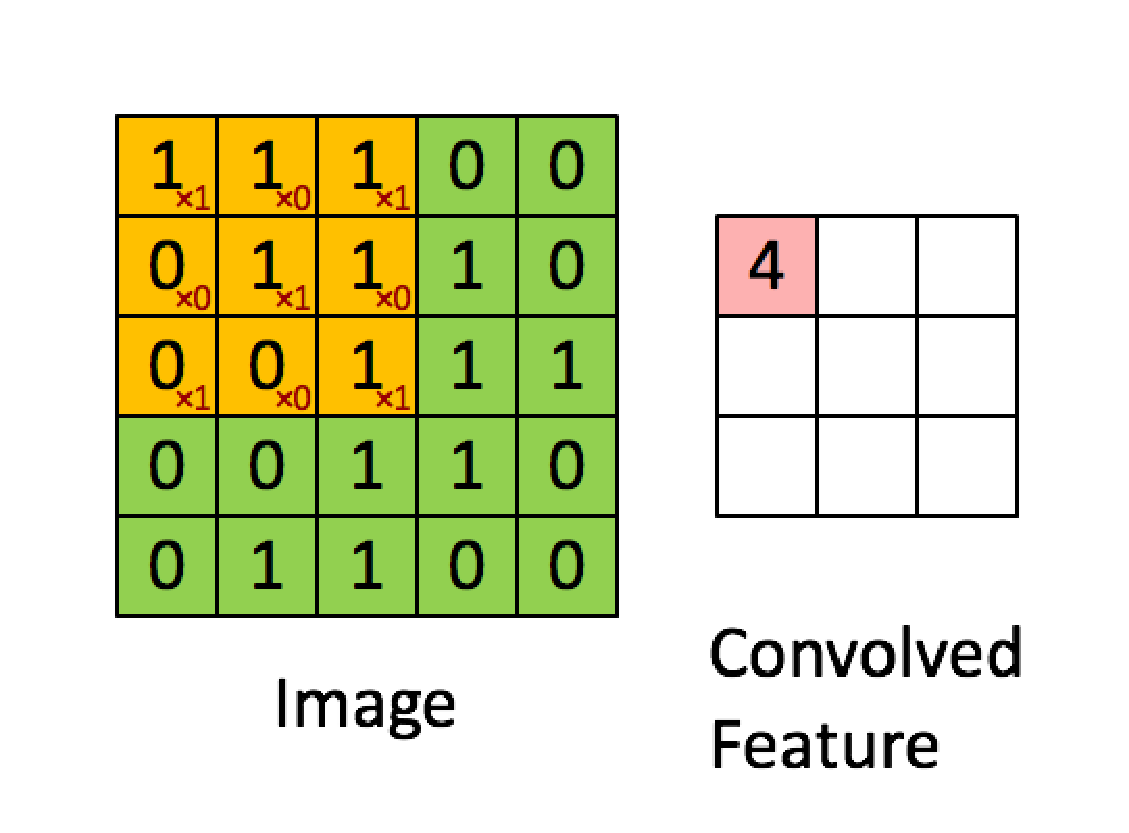
\includegraphics[scale=0.5]{./figures/convolution_example.eps}
  \caption{Example of a convolution operation at a single spatial location. The
  large yellow square represents the kernel filter. Note that no padding has been
applied here which is why the convolved feature (i.e. the response map) is
smaller.}
  \source{http://deeplearning.stanford.edu/wiki/images/6/6c/Convolution\_schematic.gif}
  \label{fig:conv_op}
\end{figure}

\para{Pooling Layers}  

As mentioned in the above paragraph, convolutional layers can perform
dimensionality reduction if no zero-padding is added to the input image.
However this job generally falls to pooling layers.

As their name suggests, pooling layers group pixels together to reduce them to a
single pixel. There are several ways to determine the value of the output pixel
and the most common one is maximum pooling which consists in outputting the
pixel in the group that has the highest value. Since this is just a static
operation, there are no learnable parameters involved. The only parameters are
the spacial extent $p$ (i.e. the width and height) of the pooling region/filter and
the stride $s$ which defines how many pixels to skip until applying the next
pooling operation. For instance, a pooling layer with $p=2$ (2x2 filters) and
$s=2$ will divide the width and height of the input image by 2 (it does not
change the depth) as can be seen in Fig~\ref{fig:maxpool}.

\begin{figure}[ht]
  \centering
  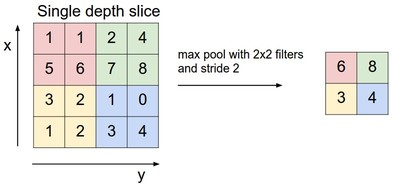
\includegraphics[scale=0.7]{./figures/maxpool.jpeg}
  \caption{example of a single max pooling operation with a $2 \times 2$ pooling
  filter and a stride of 2}
  \source{http://cs231n.github.io/assets/cnn/maxpool.jpeg}
  \label{fig:maxpool}
\end{figure}

To sum up here are the inputs and outputs of a pooling layer:

\begin{enumerate}
  \item \textbf{In}: $k$ images of size $n \times m \times d$ where $n$ is the
    width, $m$ the height and $d$ the depth of the image
  \item \textbf{Out}: $k$ responses of size $\left( \frac{n-p}{s} + 1  \right)\times
    \left( \frac{m-p}{s}+1  \right)\times d$ where $p$ is the width of the
    square pooling filter and $s$ the stride size
\end{enumerate}

\para{Fully Connected Layers}

Fully connected layers constitute the second block of DCNNs, after the block of
convolutional + max pool layers.

Unlike convolutional layers, which are locally connected (each pixel in the
response map is locally connected to a sub-region of the input), fully
connected layers have their outputs connected to \textit{every} input.

As such, the activations are simply calculated via matrix multiplication
between the inputs and their associated weights and adding a bias term before
passing this sum to an activation function (see Section~\ref{sec:activation_functions}).

It is worth noting that we can easily replace a fully connected layer by an
equivalent convolutional layer; all that must be done is to match the size of
the kernel filters to the size of the input image or vector. For instance, in
the VGG 16 \cite{RefWorks:22} network, the final convolutional layer outputs 512 feature maps of
size $7 \times 7$ which are passed on to a fully connected layer with 4096
neurons. Then we can replace this fully connected layer by a convolutional one
with 4096 filters of size $7 \times 7$

\para{Dropout Layers}

Dropout layers \cite{RefWorks:23} are a simple yet powerful regularisation technique to prevent,
overfitting. The key idea is to randomly block some neurons from connecting to
the next layer during training see Fig.~\ref{fig:dropout}. This prevents groups of neurons from
\textit{co-adapting} too much and improves the flexibility of the network which
\textit{decreases overfitting}.


\begin{figure}[ht]
  \centering
  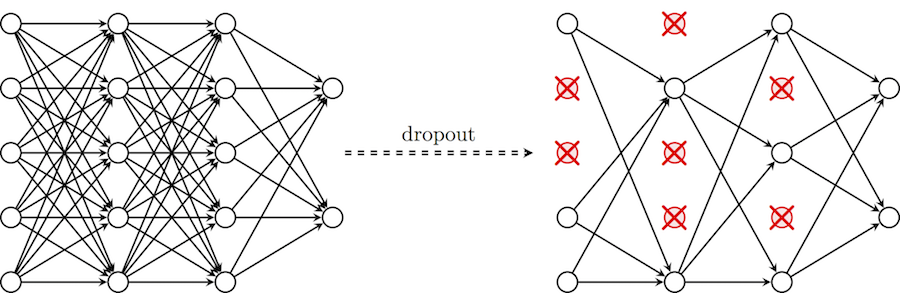
\includegraphics[scale=1.5]{./figures/dropout.png}
  \caption{example dropout layers: the crossed neurons are blocked from sending
  their inputs to the next layer}
  \source{https://cambridgespark.com/content/tutorials/convolutional-neural-networks-with-keras/figures/drop.png}
  \label{fig:dropout}
\end{figure}



\subsubsection{Activation functions}\label{sec:activation_functions}

Each trainable layer in the network also has an activation function, through
which it passes its outputs before sending them to the next layer.
The main role of activation functions is to provide non-linearity to the network.
Intuitively, this enables deep networks to better fulfil their \textit{representation
learning power}. Indeed, without these functions, deep networks (or any neural
network) would only be learning a linear combination of the input data which is
quite limiting. We now go through the main activation functions used in neural
networks.

% ---------- S I G M O I D ----------
\para{Sigmoid}\label{para:sigmoid}

The sigmoid activation function is a special case of the logistic function and
is defined as follows:

\begin{equation}
  f(x) = \frac{1}{1 + e^{-x}}
  \label{eq:sigmoid}
\end{equation}

It was a popular activation function until the arrival of the
ReLU~(\ref{para:relu}) which dealt better with the main shortcoming of this one.
Indeed, the sigmoid function squashes everything between 0 and 1 therefore, as
the absolute value of the input increases, the gradient at that point
decreases. So the gradient tends towards 0 as the input tends towards infinity.
This is called the \textit{vanishing gradient} problem and is indeed
problematic as when
performing backpropagation, the updates will not change the weights
significantly which considerably slows down training at best or prevents us to reach
a local minimum at worst.

Today, the sigmoid activation function, just like softmax (see paragraph below)
is mostly used on the very last layer of the network, to make the outputs look like
probabilities.

% ---------- S O F T M A X ----------
\para{Softmax}\label{para:softmax}
Also known as the Normalised Exponential, the softmax activation function is
defined as follows: consider the $i^{th}$ layer of a neural network and let
$\bm{z}^i$ be the vector of raw activations of this layer as defined in 
\eqref{eq:NN}, then 

\begin{equation}
  a_j^i = f(\bm{z}^i)_j = \frac{e^{z_j^i}}{\sum^{m_{i}}_{k=1} e^{z_k^i}}
  \label{eq:softmax}
\end{equation}

Where $m_i$ denotes the number of neurons in layer i.

From a probability theory point of view, the softmax activation function
calculates a probability distribution over what we can consider as $m_i$
categories. It is therefore mostly used on the very last layer of neural
networks trained to classify inputs into a single category. Therefore when
using a softmax activation function on the last layer, one assumes that these
categories are \textit{mutually exclusive}, meaning that training or test instance can
not belong to two or more categories at the same time.

% ---------- R E L U ----------
\para{ReLU}\label{para:relu}
In its simplest form, the Rectified Linear Unit \cite{RefWorks:24} for a scalar input $x$ is defined as
follows:

\begin{equation}
  f(x) = \max(0,x)
  \label{eq:relu}
\end{equation}

Variations have recently emerged such as the Leaky ReLU \cite{RefWorks:25} which is defined
as:

\begin{equation}
  f(x) = 
  \begin{cases}
    x, & \text{if}\ x >0\\
    0.01x, & \text{otherwise}
  \end{cases}
  \label{eq:leaky_relu}
\end{equation}

There are two main advantages to using ReLUs which make them the most popular
activation functions today. The first is that they significantly reduce the
likelihood of the gradient to vanish (or be extremely small) since when
$x >0$, the gradient has a constant value, unlike the sigmoid activation
function described above whose gradient becomes increasingly small as
$x$ increases. This makes learning significantly faster. The second advantage
is that using ReLU gives more sparse representations of the data as any
negative input is mapped to $0$. Sparse representations seem to be more
efficient as they encode a \textit{de facto} feature selection (if an input is
mapped to 0 then that ``feature'' is ignored) and therefore
have more potential to uncover true relationships in the data and be less
affected by noisy dependencies.

\subsubsection{Loss functions}\label{sec:loss}

Loss functions are at the core of deep neural networks as they define the
objective that we are trying to achieve. It is therefore crucial to select
the appropriate loss function depending on the task for which the network will
be trained.

\para{Mean Squared Error}\label{para:mse}

The Mean Squared Error is the most widely used loss function for regression
problems. For a data set $\left( \bm{x}_i, y_i \right)_{i=1}^N$ with $N$
examples, it is defined as:

\begin{equation}
  MSE = \frac{1}{2N}\sum_{i=1}^N (y_i - \hat{y}_i)^2
  \label{eq:mse}
\end{equation}

Where $\hat{y}_i$ is the network's prediction using input $\bm{x}_i$.

\para{Cross Entropy}\label{para:cross_entropy}

The cross entropy loss function is generally used in classification tasks when
the network outputs a probability distribution over the classes in which an
example can be categorised, either by using the softmax (\ref{para:softmax}) or the
sigmoid (\ref{para:sigmoid}) activation function.

Suppose the network outputs a probability distribution $\hat{\bm{y}}^i$ for
$m$ categories and the target
probability distribution is $\bm{y}^ii$ for $i=1\dots N$ examples. 
Then the cross entropy loss for a single example is defined as:

\begin{equation}
  H(\bm{y}^i, \hat{\bm{y}}^i) = -\frac{1}{m} \sum_{k=1}^m \bm{y}_k^i
  \log(\hat{\bm{y}}_k^i)
  \label{eq:cross_entropy}
\end{equation}

And the cross entropy loss of the whole data set is just the average of the
losses of each example in the data set as defined in Eq.
\eqref{eq:cross_entropy}.

\subsubsection{Optimisers}\label{sec:optimisers}

Now that we have overviewed the different elements that make up the structure
of a network, we must look at how to update the trainable parameters (i.e. the
weights). The key value that we use to update a parameter is the gradient of the loss function
(\ref{sec:loss}) with respect to that parameter to perform gradient descent.
This gradient,  $\Delta\bm{w}$, is computed using the backpropagation algorithm and
the most simple way to apply it to update the parameters $\bm{w}$ is as follows:

\begin{equation}
  \bm{w} \leftarrow \bm{w} - \alpha \Delta\bm{w}
  \label{eq:grad_descent}
\end{equation}

where $\alpha$, the learning rate, controls the magnitude of the updates. In this
setting, $\Delta\bm{w}$ is calculated after a forward pass of the entire
training data set. However this is computationally inefficient or unfeasible so
we use different techniques.

\para{Stochastic Gradient Descent}\label{para:sgd}

The first technique, Stochastic Gradient Descent (SGD), computes the gradient
$\Delta\bm{w}_{batch}$ w.r.t. the parameters after a forward pass of a small batch 
$(\bm{x}_{batch}, \bm{y}_{batch})$ of training examples, 
usually 128 or 256, instead of the entire dataset.
It then updates the parameters as in Eq.~\eqref{eq:grad_descent}:

\begin{equation}
  \bm{w} \leftarrow \bm{w} - \alpha \Delta\bm{w}_{batch}
  \label{eq:sgd}
\end{equation}

Since the gradients are only calculated from a small sample of the dataset,
the variance of the updates between each batch will be higher, which is why we
typically use a small learning rate of $\alpha = 0.1$ to $\alpha = 0.001$.

This technique is stochastic because we randomly shuffle the data before
dividing it into batches and calculating and applying the updates. Ideally,
this should be done before each epoch, where and epoch is defined as a pass
over the entire data set.

\para{SGD with Momentum}\label{para:sgd_momentum}

The objective of the parameter updates is to descend the gradient of the loss
function to find a good local minimum. Viewing this gradient as a hill/ravine
that we must descend, SGD with momentum uses a physical approach by
considering that we are ``rolling'' the parameter vector down that hill. As such,
Under this approach, the parameter vector has a velocity $v$ which is used to
determine its position (i.e. the update). This velocity is directly affected by
the gradients that we compute:

\begin{align}
  \bm{v} &= \mu \bm{v} - \alpha \Delta \bm{w}_{batch}\\
  \bm{w} &= \bm{w} + \bm{v}
  \label{eq:sgd_momentum}
\end{align}

Where $\alpha$ is the learning rate as in \eqref{eq:sgd} and $\mu \in (0,1]$ is referred
to as the momentum, although from a physics standpoint, it can be assimilated
to friction and is generally set to $0.9$.

SGD with momentum almost always boasts better convergence rates than vanilla
SGD. This is because as we approach a local minimum, the updates become smaller
and smaller (as the gradient tends to 0 at stationary points) so vanilla SGD
takes more time to converge to that minimum. Adding momentum on the other hand
ensures that this slow-down does not occur or is minimised.
\para{Adagrad}\label{para:adagrad}

The next set of parameter updating techniques possess the particularity of
having a \textit{per-parameter adaptive learning rate}. Adapting the learning rate can
be viewed as refining the search for a local minimum. Indeed, we first start
with a relatively large learning rate as we want to explore the gradient space
with big steps. Once a region seems promising, we would like to focus on it and
reduce size of the steps as we do not want to miss a local minimum. This can be
done by reducing the learning rate $\alpha$ when we are close to a local
maximum. While we can adapt the learning rate globally for all parameters,
recent research has focused on methods that adapt the learning rate per-parameter.
\textbf{Adagrad}, first proposed by Duchi et al. \cite{RefWorks:26}, is one of these
methods and is defined as follows: suppose we have just calculated a gradient
$\Delta\bm{w}$ for a mini batch, then the update is applied as follows:

\begin{align}
  \bm{c} &\leftarrow \bm{c} + \left( \Delta\bm{w} \right)^2
  \label{eq:adagrad_cache}\\
  \bm{w} &\leftarrow \bm{w} - \frac{\alpha}{\sqrt{\bm{c}} + \varepsilon}
  \Delta\bm{w}
  \label{eq:adagrad}
\end{align}

Here $\bm{c}$, which has the same dimensions as the parameters, acts as a cache
that stores the squared values of the previous gradients. We then divide the
learning rate $\alpha$ by the square root of $\bm{c}$ (plus some small positive
constant $\varepsilon$ to ensure that we do not divide by zero) so that the
more updates a parameter gets, the smaller its learning rate.

\para{RMSProp}\label{para:rmsprop}

One downside of Adagrad(~\ref{para:adagrad}) is that the learning rate is
monotonically decreasing which does not allow for flexibility as the learning
rate diminishes quickly.
\textbf{RMSProp} attempts to alleviate this by introducing a decay rate
parameter $\gamma$ when updating the cache $\bm{c}$. The rest is identical to
(\ref{para:adagrad}). As such the only change is that Eq.
\eqref{eq:adagrad_cache} becomes:

\begin{equation}
  \bm{c} = \gamma \bm{c} + (1-\gamma) \left( \Delta\bm{w} \right)^2
  \label{eq:rmsprop}
\end{equation}



\subsubsection{Models}\label{sec:models}

The reader is referred to \cite{RefWorks:2} (paragraph 3) for a review of existing deep learning methodologies for facial expression recognition "in-the-wild".

In terms of deep learning models, we use two pre-existing and pre-trained models, namely \textbf{VGG} \cite{RefWorks:22} and
\textbf{Inception V2} \cite{RefWorks:28}. These were fine-tuned for specific tasks on our
database (a subset of the EmotioNet database \cite{RefWorks:1})

\para{VGG 16}\label{para:vgg16}

The VGG 16 network was developed by Karen Simonyan and Andrew Zisserman from
Oxford University's Visual Geometry Group and was the runner-up in ILSVRC 2014. 
The ``16'' signifies that there are 16 trainable (weight) layers: 13 convolutional
layers and 3 fully connected layers, see Fig.~\ref{fig:vgg16}.

\begin{figure}[ht]
  \centering
  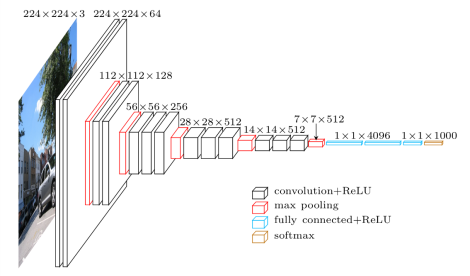
\includegraphics[scale=0.7]{figures/vgg16.png}
  \caption{structure of the VGG 16 deep convolutional network}
  \source{https://www.cs.toronto.edu/~frossard/post/vgg16/vgg16.png}
  \label{fig:vgg16}
\end{figure}

It's originality comes from the fact that it uses small kernel filters
($3 \times 3$) at each convolutional layer which are convolved with every
pixel of the input image (i.e. they use a stride of 1). Furthermore, 
the number of filters increases as we progress through the convolutional layers.
The idea behind this is to get the first layers to detect abstract features
such as lines and get the following layers to refine on that feature.

Finally all 5 max pool layers use a spacial extent of $p=2$ and a stride of
$s=2$ so that each pool layer divides the width and height of the input image
by 2 
 
\para{Inception V2}\label{para:inception_v2}

Inception networks build upon a key insight from the Network in Network
(NiN) paper \cite{RefWorks:30}, Lin et al 2014]: convolutional layers can only learn linear
combination of the inputs, to enable them to learn non linear
features, Lin et al replaced their linear kernel filters with multilayer
perceptrons. 

Researchers at Google used this insight to create the inception
module which for the first version of the network (v2) is detailed in
Fig.~\ref{fig:inception_module}

\begin{figure}[ht]
  \centering
  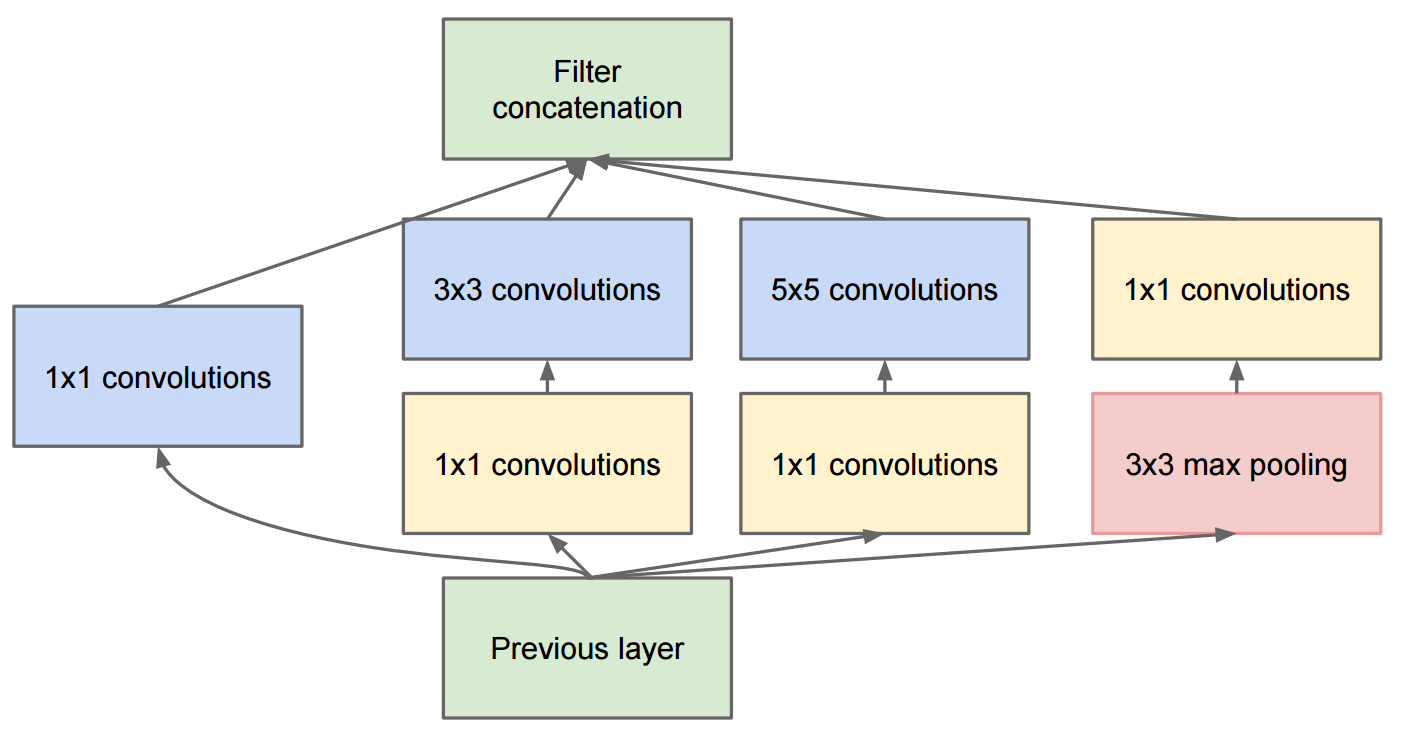
\includegraphics[scale=0.3]{figures/inception_module.png}
  \caption{The inception module with the concatenation of a pool, a $1 \times
  1$, a $3 \times 3$ and a $5 \times 5$ convolution operations}
  \source{https://i.stack.imgur.com/zTinD.png}
  \label{fig:inception_module}
\end{figure}

Indeed, the $1\times 1$ convolution layer is mathematically equivalent to a
multilayer perceptron and since it is immediately followed by a ReLU layer
(not shown in Fig.~\ref{fig:inception_module}), it allows the network to learn
non linear features. 

Furthermore, this initial $1 \times 1$ convolution layer drastically reduces
the number of trainable parameters when it is used before the $3 \times 3$ or
$5 \times 5$ convolutional layers. This therefore allows the Inception network to
combine a max pool, a perceptron, a $3 \times 3$ and a $5 \times 5$ convolution
operation into a single layer/module at no extra computational cost,
effectively allowing the network to be even deeper.

With the second version of the Inception network, which we will be using, the
inception module depicted in Fig.~\ref{fig:inception_module} differs slightly.
Indeed, the authors factorised the $5 \times 5$ convolutional layer into two
consecutive $3 \times 3$ convolutional layers as shown in
Fig.~\ref{fig:inception_v2_module}.

\begin{figure}[ht]

  \centering
  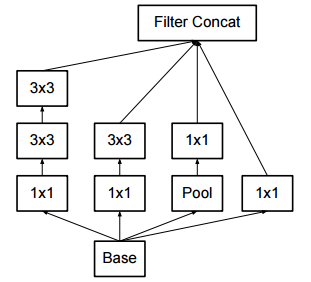
\includegraphics[scale=0.8]{figures/inception_v2_module.png}
  \caption{The inception module with the concatenation of a pool, a $1 \times
  1$, a $3 \times 3$ and a $5 \times 5$ convolution operations}
  \source{http://davidstutz.de/wordpress/wp-content/uploads/2017/03/inception\_arch\_1.png}
  \label{fig:inception_v2_module}
\end{figure}


\subsubsection{Evaluation Measures}\label{sec:measures}

Once a model has been trained, we would like to evaluate its performance on an
independent and unseen test set. To do this various measures exist to provide
meaningful insights about the quality of the model.

\para{True/False Positives and Negatives}

Consider a binary classification task, e.g. an action unit is either active
(positive class) or inactive (negative class). Then a model's prediction for
this task can fall into one four categories. If the model predicts an example
to be positive and the actual value is also positive, then it is a
\textit{True Positive} (TP). If it predicts the example to be negative when in fact
it actually is positive then this is a \textit{Type II} error and the prediction
is a \textit{False Negative} (FN).

Conversely, if the example's actual label is negative and the model predicts
it to be positive, then it is a \textit{Type I} error and the prediction is a
\textit{False Positive} (FP). Finally if the model predicts the example to be
negative when it is in fact negative, then it is a \textit{True Negative}
(TN).

Using these simple definitions, we can now define more complex evaluation
measures.

\begin{figure}[ht]
  \centering
  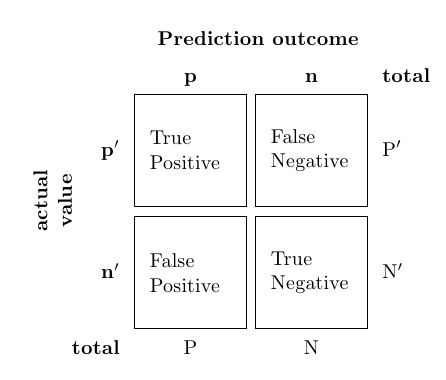
\includegraphics[scale=0.7]{figures/tf_pos_neg.png}
  \caption{The four categories a model's prediction can fall in}
  \source{https://i.stack.imgur.com/0OxEo.png}
  \label{fig:tf_pos_neg}
\end{figure}

\para{Accuracy}\label{para:accuracy}

Accuracy is the simplest and most intuitive measure, it measures the proportion
of examples that were correctly classified as positive or negative and is
defined as:

\begin{equation}
  Acc = \frac{TP + TN}{TP + TN + FP + FN}
  \label{eq:accuracy}
\end{equation}

\para{Partial Accuracy}\label{para:partial_accuracy}

Suppose the label $\bm{y}$ is as in the EmotioNet data set, i.e. an array composed of 60
entries, each corresponding to the AU of its index, which are either 1 if the
AU is active or 0 otherwise. Now suppose we also have a prediction
$\hat{bm{y}}$ of same size and also composed of zeros and ones. With normal
accuracy (\ref{para:accuracy}), if as little as one $\hat{\bm{y}}_i$ differs
from $\\bm{y}_i$, for $i=1 \dots 60$, then the prediction is assumed to be
incorrect as a whole, as it does not match the label exactly, entry for entry.
This is not desirable when the classes are not mutually exclusive as the other
entries (e.g. the other AUs) are correctly classified. We are therefore
interested in the proportion $P_i$ of classes (e.g. AUs) that are correctly
predicted within a single label $\hat{\bm{y}}^i$:

\begin{equation}
  P_i = \frac{1}{m}\sum_{k=1}^m I(\hat{\bm{y}}^i_k, \bm{y}_{k^i})
  \label{eq:partial_accuracy}
\end{equation}

Where $m$ is the number of classes and $I(a, b) = 1$ iff $a = b$ and 0
otherwise. We then take the average of the $P_i$ over $i=1\dots N$ to output the average
partial accuracy of the model over a test set of $N$ examples.


\para{Recall}\label{para:recall}

Recall measures the proportion of \textit{actually} positive examples that where
\textit{predicted} as being positive and is defined as:

\begin{equation}
  Recall = \frac{TP}{TP + FN}
  \label{eq:recall}
\end{equation}

Note that one can achieve a Recall of 1 (the highest value possible) by
predicting every example as positive.

\para{Precision}\label{para:precision}

Precision measures the proportion of examples that \textit{actually} are positive
within the set of examples that were \textit{predicted} to be positive. It is
defined as:

\begin{equation}
  Precision = \frac{TP}{TP + FP}
  \label{eq:precision}
\end{equation}

\para{F1 Measure}\label{para:f1_measure}

The F1 measure is the harmonic mean of the recall \eqref{eq:recall} and the
precision \eqref{eq:precision} and is defined as:

\begin{equation}
  F1 = 2\times \frac{1}{\frac{1}{recall}+\frac{1}{precision}} = 2 \times
  \frac{precision \times recall}{precision + recall} 
  \label{eq:F1}
\end{equation}

Intuitively, it measures the balance between precision and recall, with an F1
score of 1 signifying perfect balance (i.e. both precision and recall are 1).

\clearpage
\section{EmotioNet Database}
 
\subsection{Downloading}

In order to use less space, the authors of the EmotioNet database do not offer
a direct download of the 25k images. Instead, they provide an xlsx file containing one line per image which consists of 61 columns: the first column corresponds to the URL of the image and the next 60 columns correspond to the 60 AUs in ascending order. To download the database, one must therefore read this file line by line, get the image at the specified URL and store it in a file. 

\subsubsection{Reading the xlsx file}

Python does not natively support the reading of xlsx files, and even though third party packages such as \textbf{openpyxl} by Eric Gazoni and Charlie Clark exist, we chose to convert the xlsx file containing the URLs and labels to a CSV file as these are easily readable in Python. One problem arose using this method, some URLs (less than 15) contained commas, meaning that the URL was split up into two or more columns which shifted the index of the AU values, thus giving an invalid label to the associated image. To remedy to this situation, we simply deleted all the commas from the URLs.

\subsubsection{Downloading the image}

Once we have retrieved the URL, we can get the raw image over the Internet by using the \textbf{urllib} library. This did not come without some complications as 2,760 images were not downloaded due to the errors listed below:

\begin{itemize}
\item HTTP 404 (Not Found) error: 1,726 URLs
\item HTTP 400, 401, 403, 410 errors: 205 URLs
\item HTTP 500, 502, 503, 504 errors: 102 URLs
\item HTTP 301, 302 errors: 20 URLs
\item Name or service not known: 500 URLs
\item Connection timed out: 109 URLs
\item Connection reset by peer: 17 URLs
\item Connection refused: 16 URLs
\item No route to host: 10 URLs
\item Certificate verify failed: 14 URLs
\end{itemize}

The \textit{Name or service not known} errors can be caused by the lack of an internet connection which can occur when downloading via Wi-Fi. Because of this, some valid URLs will not be accessed to download an image. To solve this problem, we keep track of which images remain to be downloaded by taking all the URLs and removing those that were already downloaded as well as those that led to an error and launch the download script again. To keep track of the erroneous URLs, each time an URL leads to an error, it is stored along with its error in a text file and to construct the list of already downloaded images, we just list the files present in the specified download directory.

\subsubsection{Storing the image}

Storing the fetched raw image implies creating a file and more importantly naming it in such a way that using this name, we can retrieve the associated label (AU values) from the xlsx file. We initially used an URL parser to extract the query component of the URL which should consist of the name of the image (e.g. image.jpeg). However, it turns out that this query component can also have a parameter component (e.g "?size=200x200" in HTTP://www.foo.com/bar/image.jpeg?size=200x200). So converting the URL into a file name based solely on the query component of the URL meant that two different URLs/images could lead to the exact same file name when we require this \texttt{url\_to\_filename} function to be a bijection in order to be able to retrieve the associated label from the xlsx file.

We therefore abandoned this method and just used the URL with a couple of preprocessing steps as file name. The preprocessing steps consisted in removing full stops from the URL and replacing forward slashes with underscores as they would otherwise be understood as directories by the file system. Additionally, we determine the type of the ray image (e.g. png, jpeg, gif ...) and append it to the file name. Finally, file names cannot be longer than 250 chars on most systems so we truncate the beginning of URLs that violate this limit.

\subsection{Converting to TFRecords}

TFRecords is the standard recommended file format to store data that will be used by a TensorFlow network or Graph. It is based on Google's Protocol Buffers which are language and platform agnostic object serialisation mechanisms. 

Converting a data set to a set of TFRecord files is no easy task, but thankfully TensorFlow provides a script, \texttt{build\_image\_data.py}, that does just that and only needed a few modifications to adapt it to the nature of our data set. Indeed, this script provided by TensorFlow was used to convert the images of the CIFAR-10 database and relied on a special organisation of the data to assign labels: one eponymous subdirectory should be created for each image category (label) and all the images of that category should be placed into that subdirectory (e.g. and image of a cat would be in the /dataset/cat/ subdirectory). However this mechanism does not apply in our case since it assumes that the categories are mutually exclusive (one image cannot be categorised as a cat and a dog at the same time) to partition the data set into subdirectories, whereas in our case, an image can have multiple active AUs at once.

So we had to change the way the script assigned labels to images by constructing a dictionary of URLs to labels using the xlsx data file and then using the file name of the image to look up its label in this dictionary. We also had to change the way the label was stored in the TFRecord as it now consist of an array of \texttt{int64} rather than a single \texttt{int64}. Finally, the script converts any PNG image to JPEG for consistency, however, it does not handle other image types such as GIF so we added the necessary logic to convert GIFs to JPEG images.

The script then takes care of multi-threading for efficiency and outputs a training and a validation TFRecord file, both split into a number of user-specified shards.

\subsection{Extending TF-Slim datasets}

Having downloaded the database and converted it to TFRecord format, we now
extend the TF-Slim datasets to incorporate ours. This has many advantages as
TF-Slim then takes care of creating a data provider for our models and more
importantly, it allows us to easily reuse TF-Slim's generic training and
evaluation scripts.

In order to do this, we created a new file in \texttt{/slim/datasets/} called \texttt{images.py} 
which returns an instance of a TF-Slim Dataset class, customised for our dataset. 
We then add this instance to the \texttt{dataset\_factory} file's dictionary.
Our dataset can now be accessed using the
\texttt{dataset\_factory.get\_dataset()} method which only requires the name of
the dataset, the path to the actual data and the name of the split to use (one
of 'train' or 'validation'). This means that we can easily change data sets,
should we add some in the future and makes our training and evaluating system
more modular.

\subsection{Annotating Valence and Arousal}

As mentioned in section (\ref{sec:databases}), this database was annotated by human annotators
on Action Unit presence/absence only. However, we are also interested in
valence and arousal values as it is strongly believed that the presence or absence of
AUs is correlated to the valence and arousal of the emotion that can be
interpreted from a facial expression.

As such, one of the major tasks, is to first annotate the 21,500 images that
were downloaded with both valence and arousal. This is1 done using a tool
available for research purpose only and developed by J. Kossaifi, 
G. Tzimiropoulos, S. Todorovic and M. Pantic. This tool was designed to
annotate videos, not large image data sets, so we first divided the 21,500
images into 21 videos of 1000 frames and a 22nd video of 500 frames. You then
load up a video and start annotating the frames for valence. Once all the
frames of the video are annotated with valence, we annotate them with arousal
and move on to the next video.

\clearpage
\section{Action Unit Prediction}

The first deep learning task consisted in fine-tuning a model for AU
classification on the EmotioNet data set that was downloaded in the previous
section. We used two different pre-trained models, VGG 16 and Inception V2, to
this end.

\subsection{Adapting training scripts}

\subsubsection{Duplicating the Logits}

The \texttt{tensorflow/models/slim} source code provides a generic training
script to train or fine-tune VGG and Inception models on different data sets.
This training script offers considerable flexibility as virtually any training
parameter can be specified using and exhaustive set of flags.

However, this training script expects 1-dimensional labels (e.g. 'Car') when
our data has 2-dimensional labels. This caused problems when trying to compute
the loss function as there was a mismatch between the logits (the outputs of
the network) and the labels. Indeed, the script performs one-hot encoding on
the labels which adds a dimension and transforms each label into a
$60 \times 60$ matrix whereas the logits are a vector of $1 \times 60$. To
solve this problem, we simply duplicated each logit by the number of classes
(60) so as to obtain a $60 \times 60$ matrix with identical rows (equal to the
original logit). 

This works from a mathematical view point as we are using the softmax cross
entropy loss function (see (\ref{para:cross_entropy})) and so each entry in this new logit matrix will be
multiplied by its corresponding entry in the one-hot label matrix. But since it
is one-hot, only one entry per row is 0 which means that the one-hot label
matrix effectively selects the appropriate logit entry and disregards the
others by multiplying them by zero.

\subsubsection{Cleaning the Labels}\label{sec:cleaning}

In the labels provided by the data set, each action unit can take on 3 values:
0 for inactive, 1 for active and 999 for undefined. However, we would like them
to only take on 2 discrete values: 0 and 1. As such, it was necessary to
preprocess the labels before feeding them to the loss function in order to
replace every 999 by a 0. We will later see that this does not lead to
desirable results.

\subsubsection{Changing the final activation function}

Originally, the training script used \texttt{softmax\_cross\_entropy\_with\_logits}
as its loss functions. The unscaled logits were therefore passed through a softmax (\ref{para:softmax}) 
function before computing their cross entropy. This lead to some very poor
results with the training loss growing to numbers greater than $10e^6$. This is
because the softmax function calculates the probability of the training
example/image to be one of the classes, therefore assuming that these classes
are mutually exclusive so that that the image can not belong to two classes at
the same time. However, this is not the case for our data set as images can
have multiple AUs/classes active at the same moment. As such, the probabilities
calculated by the softmax function will be low (as there is no clear
``winner'' class) which gives large values when we take the negative log of
these probabilities in the cross entropy. 

Therefore, the \texttt{softmax\_cross\_entropy\_with\_logits} loss function is
not adapted to our situation. Instead, we must treat each action unit as an
individual binary (is it activated or not, i.e. 1 or 0 respectively)
classification task. This can easily be done by replacing the softmax
activation function by a sigmoid activation function (\ref{para:sigmoid}). Indeed, the sigmoid
function does not normalise each value in the logit array with respect to the
others, thus treating each class as independent of one another. As such all
that had to be done was to replace the current loss function with the following
\texttt{sigmoid\_cross\_entropy\_with\_logits}. This also mean that it was
unnecessary to duplicate the logits before passing them to the loss function as no
one-hot encoding of the labels is necessary.

\subsection{Prediction of 60 Action Units}\label{sec:pred_60_au}

We started the action unit prediction task with the whole set of action
units. That is, for each training image,  we learn to predict if each of the 60
AUs are either active or inactive. Note that as discussed in
(\ref{sec:cleaning}) we marked the AUs labelled as occluded as inactive. Though
this is should not be done, it was impossible to simply remove any example
whose label contained a '999' as we would be left with an empty data set since
each label contained at least one AU marked as '999'.

\subsubsection{Fine-tuning}

The training consisted in fine-tuning the VGG 16 and Inception V2 (see
\ref{sec:models}) on a data set split of 15,000 examples.
For the VGG 16 models, this meant training the weights of
the final three convolutional layers whilst freezing the remaining
convolutional layers whereas for Inception V2, this meant training the final
logits layer whilst freezing the rest of the network. 

Both networks were trained using the RMSprop optimiser (\ref{para:rmsprop})
using a decay rate of $\gamma = 0.9$ and a momentum parameter of 0.9 as well.
We also used an initial learning rate of $0.01$ in both cases, with an
exponential decay using a decay factor of $0.94$ and an interval of 2 epochs
between two decays of the learning rate. The batch size was set to $32$ and
finally a weight decay of $0.00004$ for the L2 regularisation term. 

We carried out the fine-tuning for $5,000$ steps which amounts to about
$11$ epochs.

\subsubsection{Evaluation}\label{sec:eval_60_au}<++>

Evaluation was carried out on a separate and independent data set split of 6400
images. For each model, we report the total accuracy, the partial accuracy, the recall,
the precision,  the F1 measure and the AUC (see section \ref{sec:measures}) as
shown in Table~\ref{tab:eval_au_60}.

\begin{table}
  \centering
  \begin{tabular}{|l|l|l|}
    \hline
    \backslashbox{Measure}{Model} & VGG 16     & Inception V2 \\
    \hline
    Total Accuracy                & 0.97710675 & 0.97671616\\
    Partial Accuracy              & 0.97710687 & 0.97671622\\ 
    Recall                        & 0          & 0.12441715\\
    Precision                     & 0          & 0.46832192\\
    F1 Score                      & 0          & 0.19660347\\
    AUC                           & 0.5        & 0.56055355\\
    \hline
  \end{tabular}
  \caption{Evaluation measures for AU prediction/classification on the full set
  of AUs (AUs 1 to 60)}
  \label{tab:eval_au_60}
\end{table}

The first figure that strikes us when looking at the results listed in
Table~\ref{tab:eval_au_60} is the abnormally high total and partial accuracy
for both networks, as well as how close these accuracies are. Such high
results, coupled with low recall and precision should alarm us and after a
quick analysis of the labels provided with this data set, one can understand
why we obtain such high figures. 

Indeed, out of the 60 action units available, only 11 of them (AUs 1,2, 4, 5,
6, 9, 12, 17, 20, 25 and 26) were truly annotated. These AUs correspond exactly
to those that were annotated in the DISFA \cite{RefWorks:17} database with the only
difference being that this database was annotated for an additional AU, namely
AU 15. The remaining 49 AUs were marked as '999' (as being occluded) for almost
every image of the test and training set. Furthermore, since we ``clean'' the
labels as described in (\ref{sec:cleaning}), these action units are marked as
inactive just before training. The model therefore just has to predict a value
of 0 for these AUs, which it can do very accurately since these AUs are almost
always 0 after cleaning.

This lack of variance in the labels can explain the high accuracy displayed by
both VGG 16 and Inception V2 as both networks do not have to learn much.
Moreover, since most of the entries (49 out of 60) of each label will be 0
(after cleaning), there is a heavy bias towards that value which means that the
models are more likely to predict a 0 instead of a 1. As such, the low recall
and precision (and thus the low F1 score) result from the fact that 0s are
considered as negatives and 1s as positives. Indeed, this suggests that there
are many true negatives/false negatives, since many 0s/1s are
correctly/incorrectly predicted as 0s and also that
there are very few true positives/false positives as almost no AUs are predicted to be 1
(active). This is confirmed by Table~\ref{tab:tf_pos_neg_60_au}.

We do note that the Inception V2 model copes better than the VGG 16 model  with this lack of variance
and imbalance of ``classes'' within the labels as it has around 1,000 true
positives. However, this figure is insignificant when compared to the number of
true negatives which we have artificially created by cleaning the labels.

\begin{table}
  \centering
  \begin{tabular}{|l|l|l|}
    \hline
    \backslashbox{Measure}{Model} & VGG 16 & Inception V2 \\
    \hline
    \hline
    True Positives                & 0       & 1,094\\
    \hline
    False Positives               & 0       & 1,240 \\
    \hline
    True Negatives                & 375,209 & 373,967 \\
    \hline
    False Negatives               & 8,791   & 7,699 \\
    \hline
  \end{tabular}
  \caption{Reporting the number of True/False Positives/Negatives for VGG 16
  and Inception V2 trained to predict action units for the full set of action
units}
  \label{tab:tf_pos_neg_60_au}
\end{table}

\subsubsection{Conclusion}

From this initial approach to fine-tuning a deep learning model to predict if
an action unit is active or not on the full set of 60 action units, we conclude
that we cannot use this full set of AUs. Indeed, too many of them are marked as
being occluded which created a significant class imbalance and invariance once
we have ``cleaned'' the labels. As such, it would be better to restrict the
number of AUs we would like to predict so as to limit the number of AUs marked
as occluded.

\subsection{Predicting 11 Action Units}

Following the previous conclusion, we limit ourselves to the following 11
action units:

\begin{enumerate}
  \item AU 1: Inner Brow Raiser
  \item AU 2: Outer Brow Raiser 
  \item AU 4: Brow Lowerer
  \item AU 5: Upper Lid Raiser
  \item AU 6: Cheek Raiser
  \item AU 9: Lid Tightener 
  \item AU 12: Lip Corner Puller
  \item AU 17: Chin Raiser
  \item AU 20: Lip Stretcher
  \item AU 25: Lips Part
  \item AU 26: Jaw Drop
\end{enumerate}

Coincidently, these 11 AUs correspond to those that have been annotated in the
DISFA database (minus AU 15). They were chosen for the sparsity of 999/occluded
entries in their labels. Indeed, having eliminated all the other action units,
we then eliminate any image that has one of the AUs listed above marked as 999.
After carrying out this cleansing, we are left with a new dataset, which we
will call EmotioNet-11AU, composed of 10,282 training and 4,424 test images.

\subsubsection{Fine-tuning}

We can now conduct a proper fine-tuning of the VGG 16 and Inception V2 models.
As in the previous section, we use the RMSprop (\ref{para:rmsprop}) optimiser
with a decay rate of $\gamma=0.9$ and a momentum of 0.9. The learning rate also
has the same exponential decay with a decay factor of $0.94$ and the same
interval of $2$ epochs between 2 successive decays. Finally, the weight decay
for the L2 regularisation term is the same at 0.00004.

However, perform multiple trainings whilst first varying the batch size and
then the initial learning rate so as to select the best hyper-parameter.

\para{Batch Size Selection}\label{para:batch_size_au11}

We first wish to select an appropriate batch size so that the training
has good convergence. To do so, we train the Inception V2 model for 20,000
steps, using the following batch sizes: 32, 64, 128, 256 and record the
evolution of the training loss as we progress through the number of steps. 

The results are presented in Fig.~\ref{fig:batch_size_11au} and show that using
a small batch size is not efficient as the training loss actually increases
during the first 2,500 steps before declining in a linear fashion. As we
increase the size if the batch size, the training loss decreases more for a
given number of steps. This trend culminates with the maximum batch size we
have tested, 256, as the training loss decreases exponentially up to step 4,000
where it hits a plateau of about 0.275 which batch size 128 reaches at step
8,000 and batch size 64 at step 16,000. We do note however that, since 256 is
twice as much as 128 and 4 times 64, and the corresponding number of steps
follow this proportion, using a batch size of 64, 128 or 256 will require a
similar number of epochs to reach the plateau training. 
This is not true for a batch size of 32. 

We therefore chose a batch size of 128 as a compromise between the number of
steps required to converge and the time (in seconds) each of these steps take.

Concerning the VGG 16 model, we used a batch size of 32 as anything above that
caused our server to run out of GPU memory due to the large number of parameter
that this model has.

\begin{figure}[ht]
  \centering
  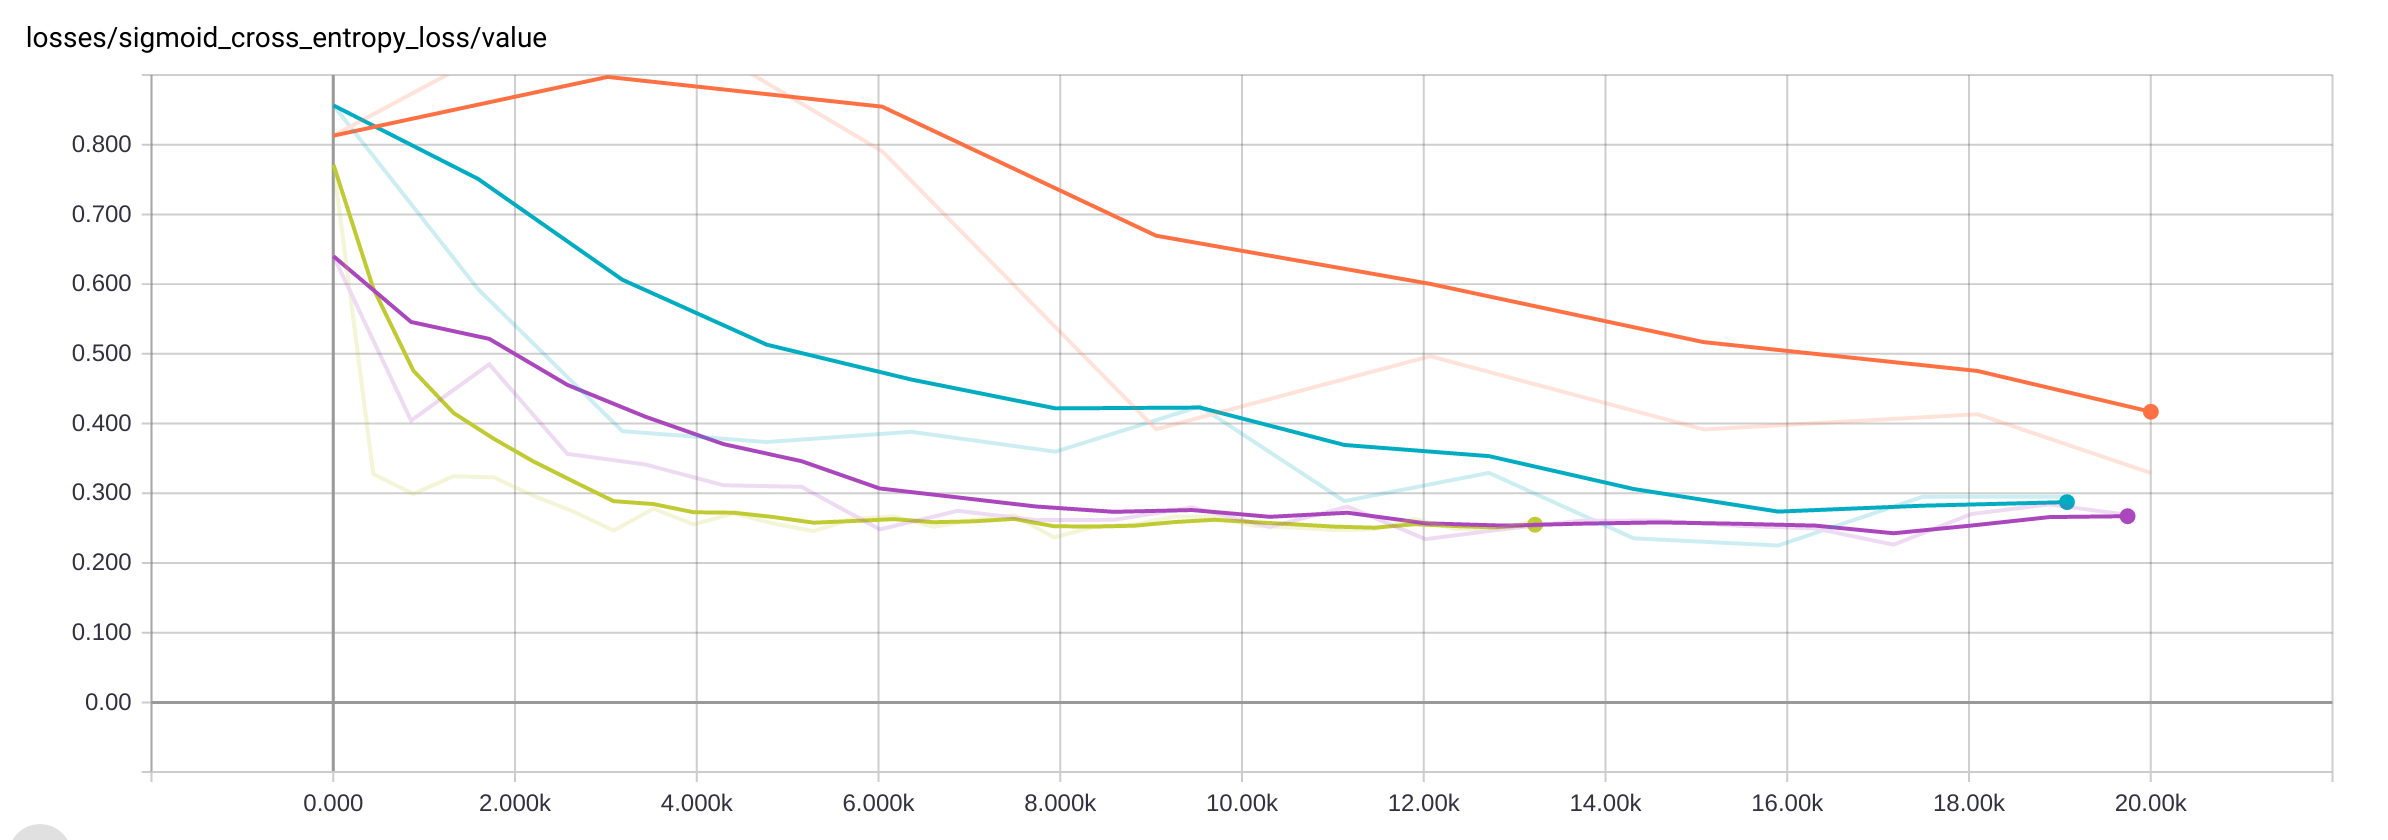
\includegraphics[scale=0.2]{figures/batch_size_11au.png}
  \caption{Training loss for different batch sizes: 32=orange, 64=cyan,
  128=magenta, 256=green}
  \label{fig:batch_size_11au}
\end{figure}


\para{Initial Learning Rate Selection}

Having picked a batch size of 128, we now focus on selecting an effective
initial learning rate. To do this we train 3 Inception V2 models with initial
learning rates of 0.1, 0.01 and 0.001 respectively for 3,500 steps.
Fig.~\ref{fig:learning_rate_au11_inception} shows the training loss against the
number of steps for these three learning rates. Clearly using an initial
learning rate of 0.1 leads to an unwanted increase of the training loss as we
progress though the steps and so should be avoided. Using an initial learning
rate of 0.1 or 0.001 leads to the similar type of linear decrease of the training loss,
with the learning rate 0.001 boasting the best results. We therefore select
$\alpha=0.001$ as our initial learning rate for the Inception V2 model.


\begin{figure}[ht]
  \centering
  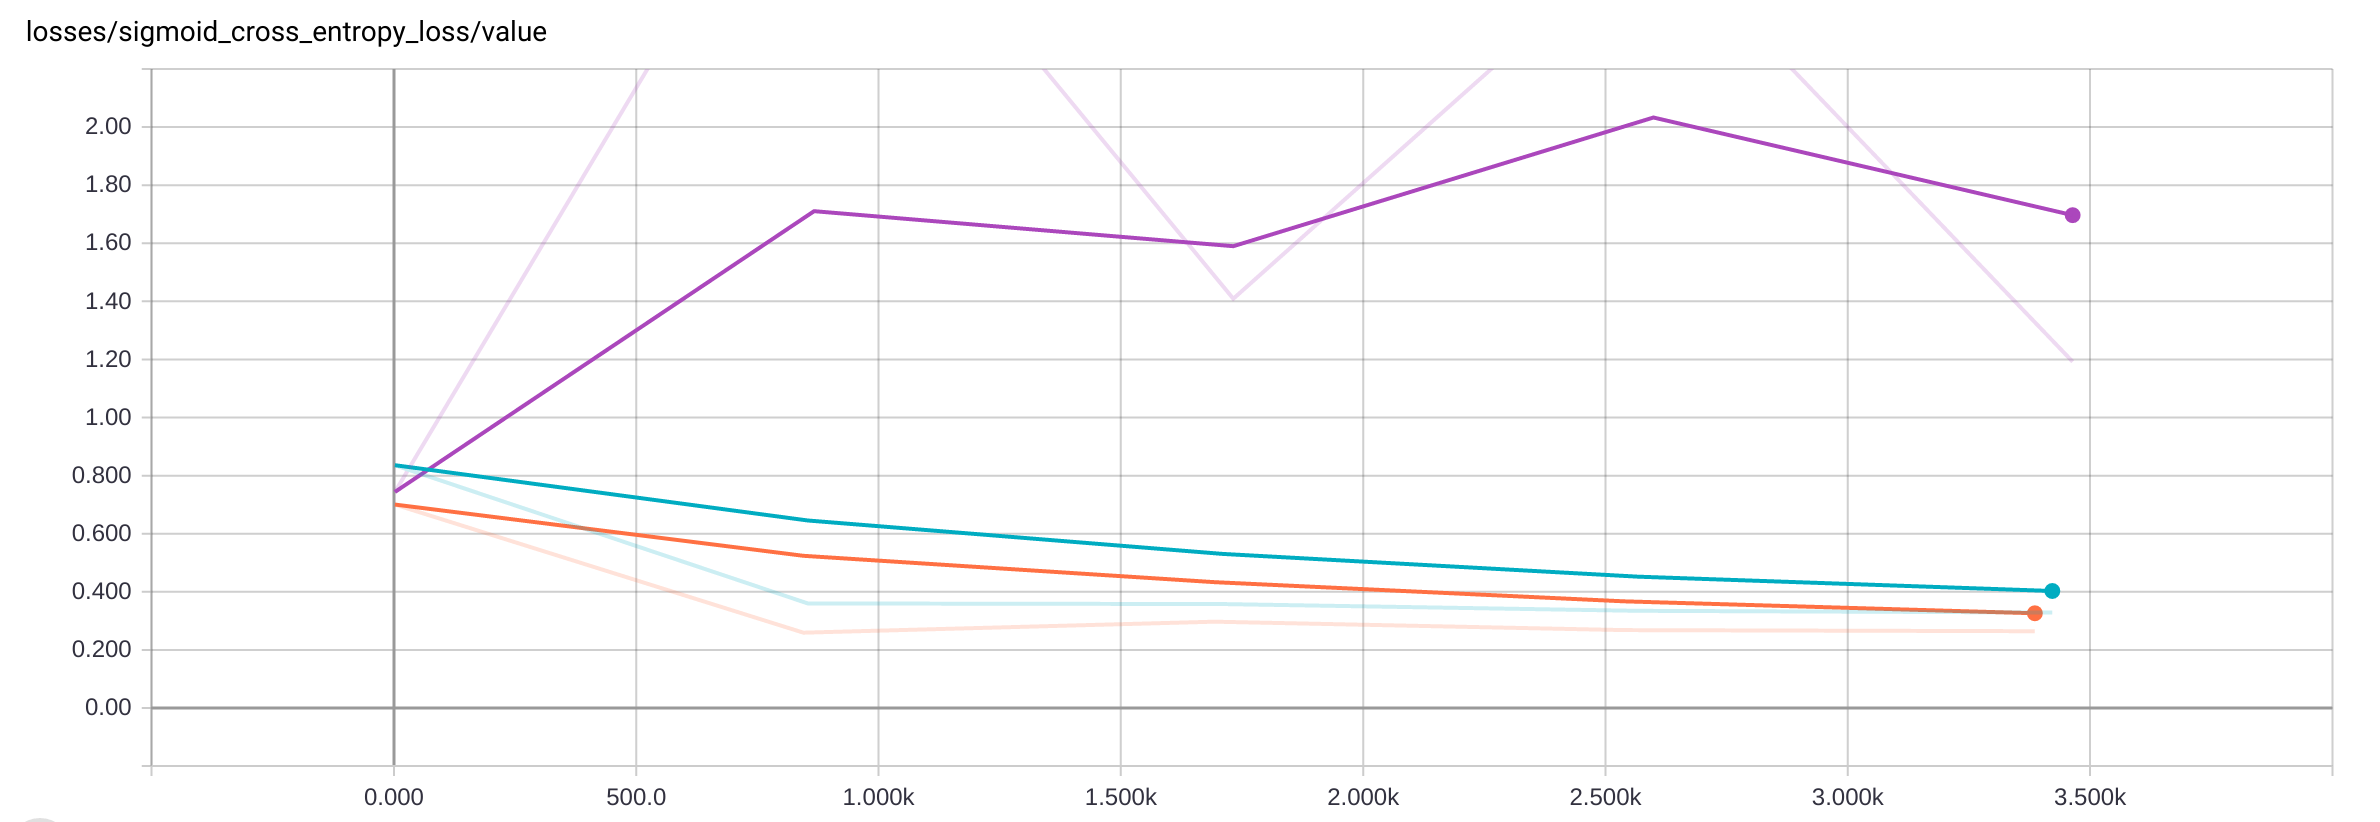
\includegraphics[scale=0.2]{figures/learning_rate_au11_inception.png}
  \caption{Training loss using Inception V2 model with the following different
    initial learning rates: 0.1=purple, 0.01=cyan,
  0.001=orange}
  \label{fig:learning_rate_au11_inception}
\end{figure}


For the VGG 16 model, having selected a batch size of 32, we now perform the
same experiment as above by training three VGG 16 model with 0.1, 0.01, 0.001 as
initial learning rates respectively. The training loss of these three models is
plotted in Figures \ref{fig:learning_rate_01_11au_vgg16},
\ref{fig:learning_rate_001_11au_vgg16} and
\ref{fig:learning_rate_0001_11au_vgg16} respectively. From these, we clearly
see that the smallest initial learning rate, $\alpha = 0.001$ should be picked
as the other two result either bad convergence for $\alpha=0.01$ or extremely
high training loss for $\alpha=0.1$. Therefore, as with the Inception V2 model,
we select $\alpha=0.001$ as our initial learning rate.

\begin{figure}[ht]
  \begin{subfigure}[b]{1\textwidth}
    \centering
    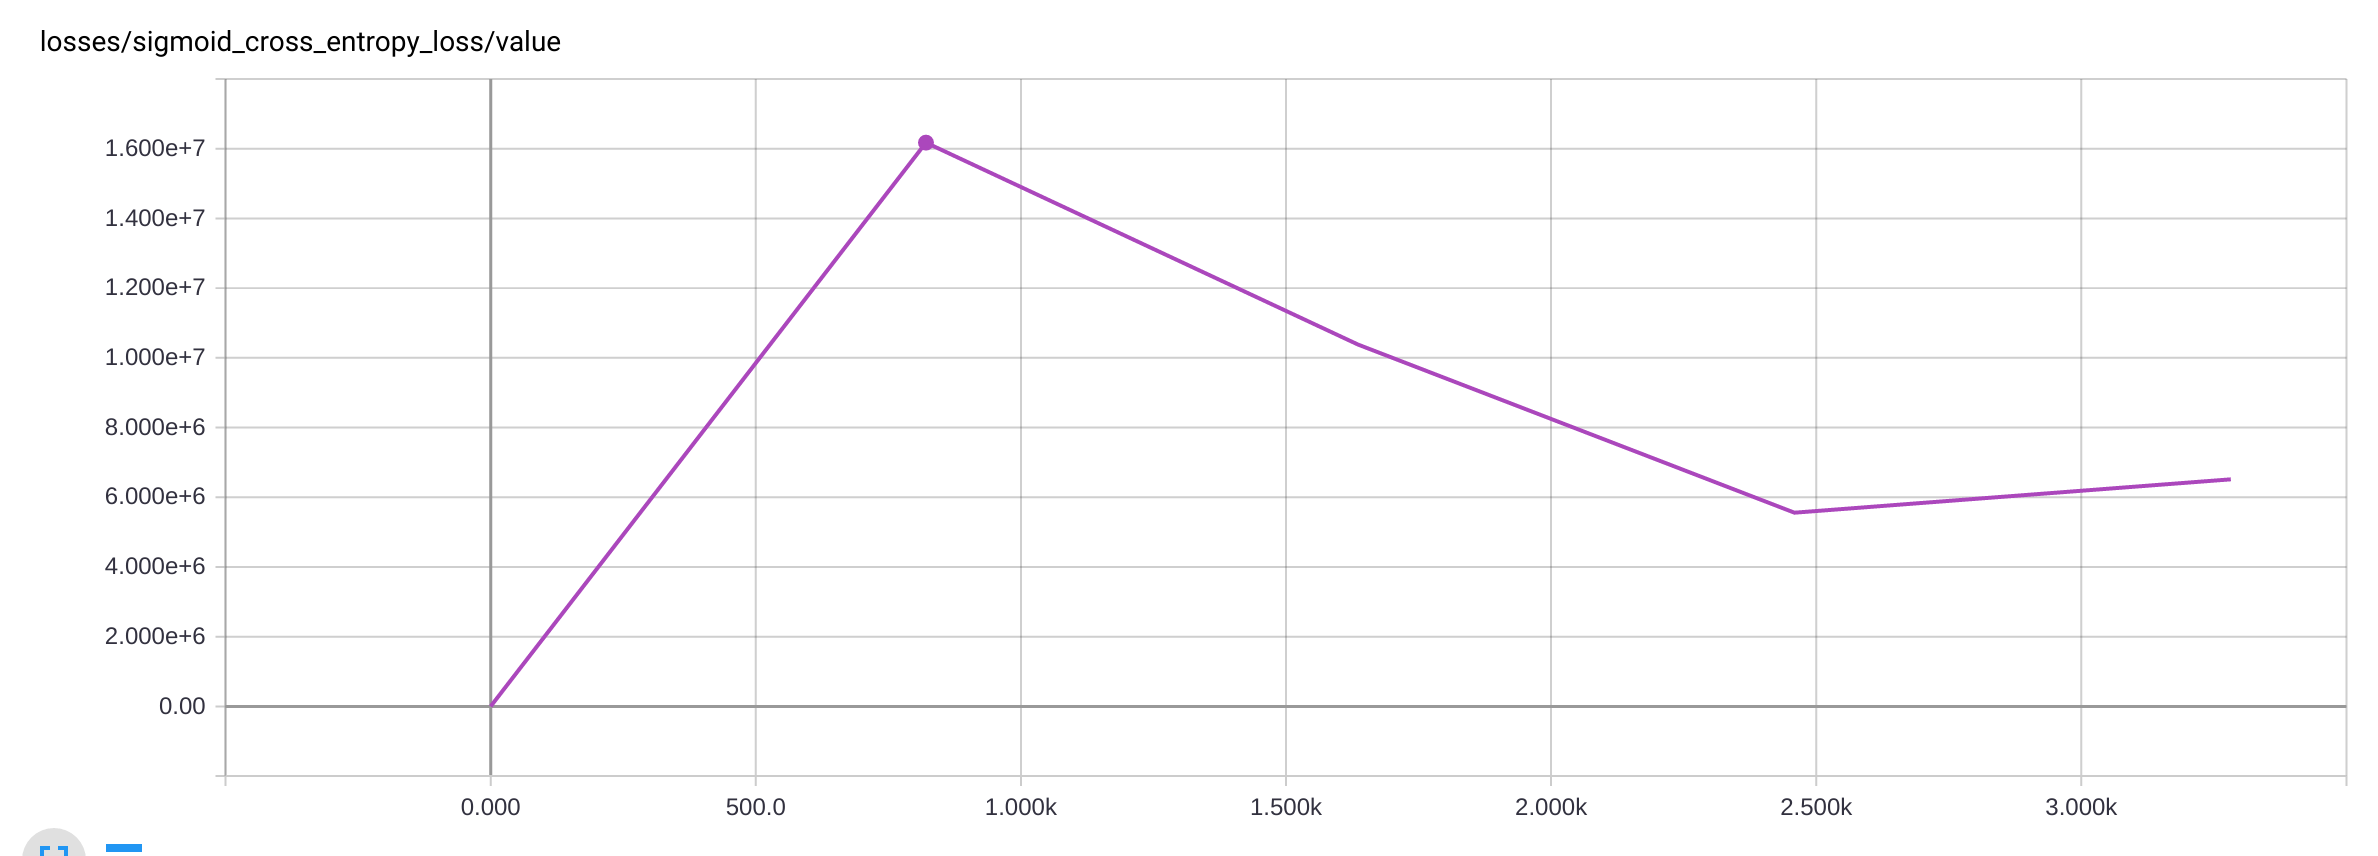
\includegraphics[width=1\linewidth]{figures/learning_rate_01_11au_vgg16.png}
    \caption{$\alpha=0.1$}
    \label{fig:learning_rate_01_11au_vgg16}
  \end{subfigure}
  
  \begin{subfigure}[b]{1\textwidth}
    \centering
    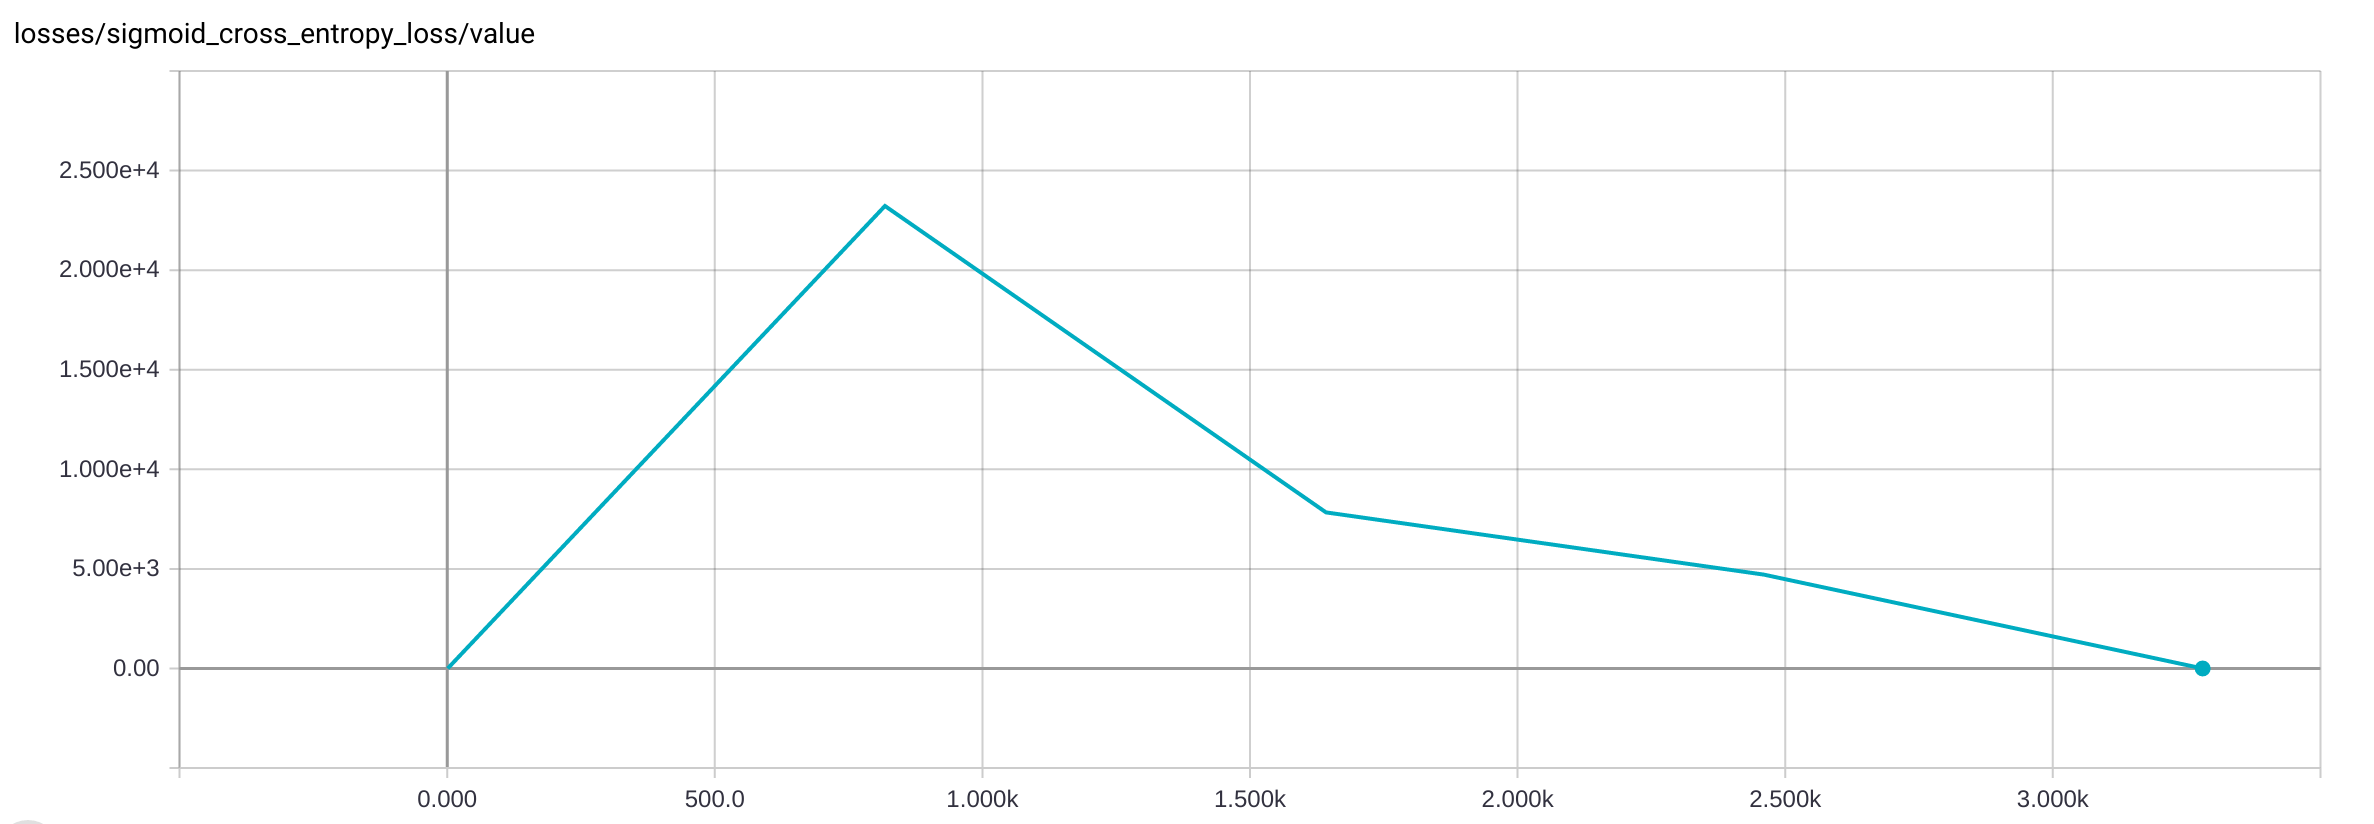
\includegraphics[width=1\linewidth]{figures/learning_rate_001_11au_vgg16.png}
    \caption{$\alpha=0.01$}
    \label{fig:learning_rate_001_11au_vgg16}
  \end{subfigure}
  
  \begin{subfigure}[b]{1\textwidth}
    \centering
    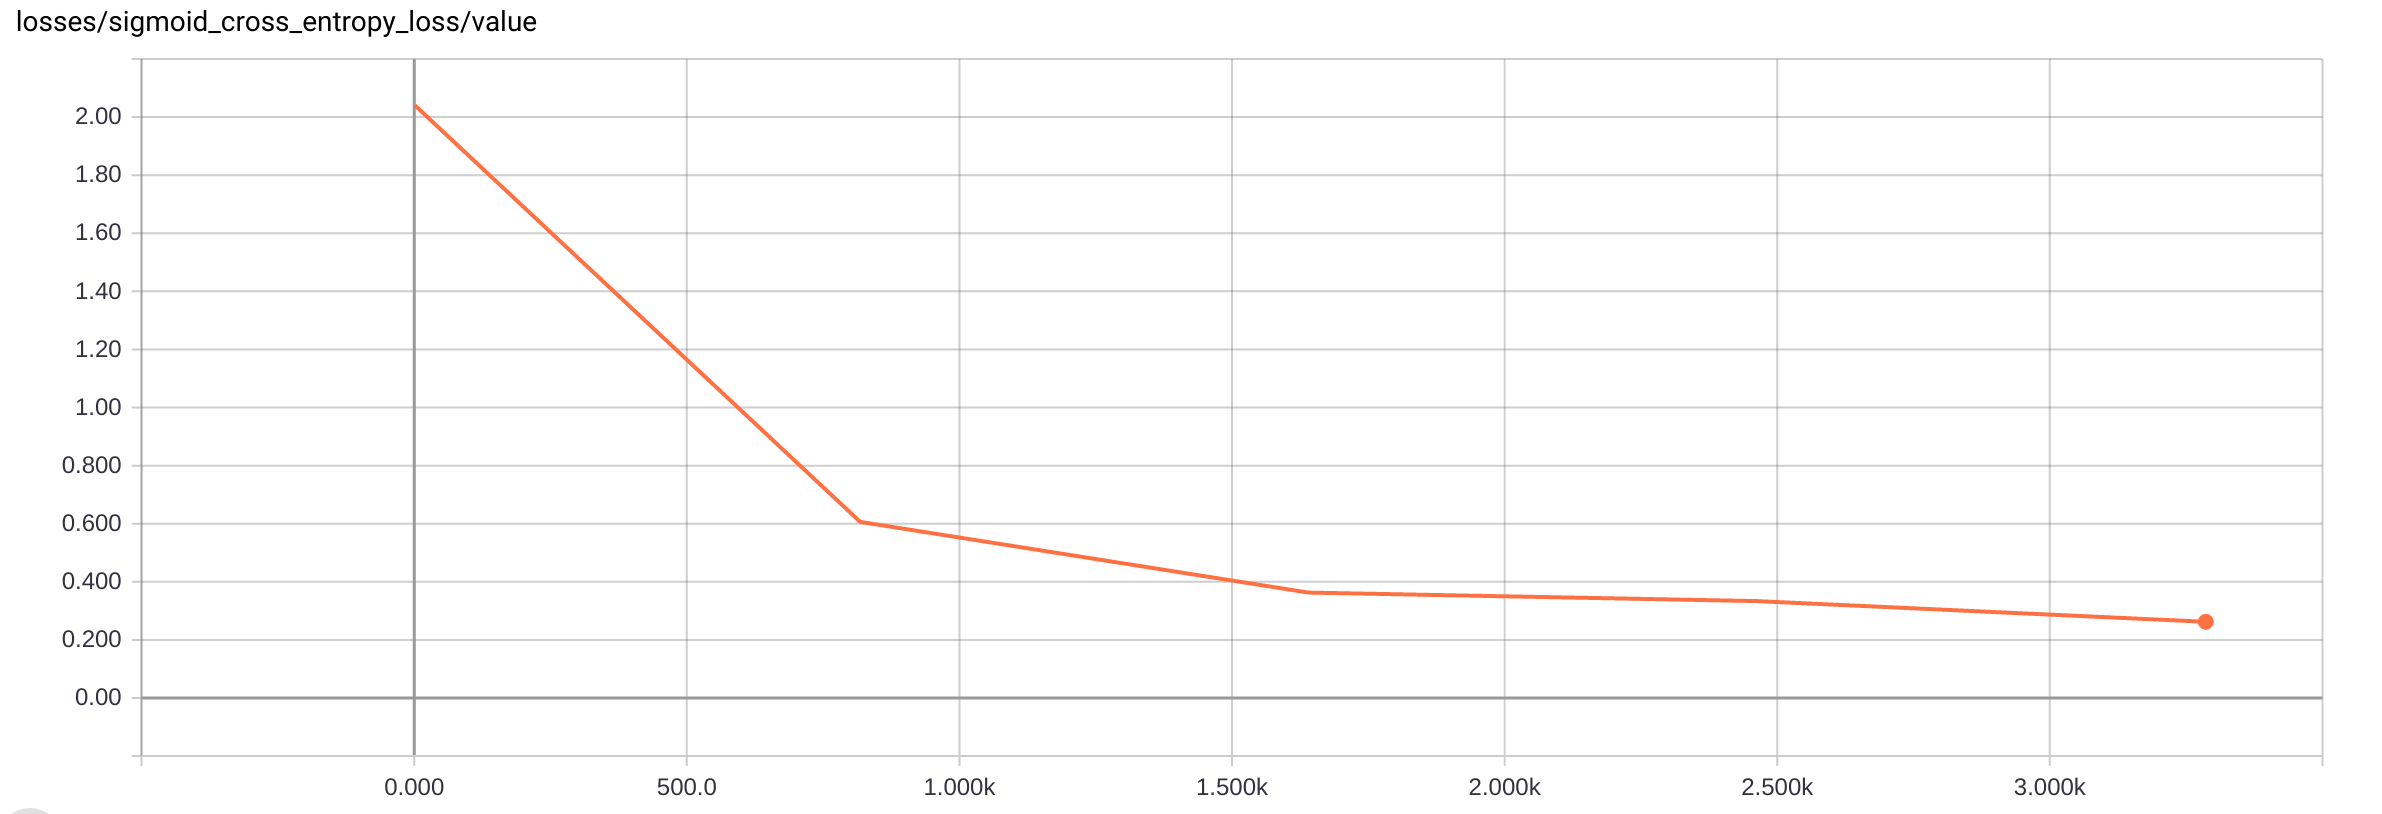
\includegraphics[width=1\linewidth]{figures/learning_rate_0001_11au_vgg16.png}
    \caption{$\alpha = 0.001$}
    \label{fig:learning_rate_0001_11au_vgg16}
  \end{subfigure}

  \caption{Training loss against number of steps for the VGG model for varying
  initial learning rate $\alpha$}
\end{figure}

\subsubsection{Evaluation}\label{sec:eval_11_au}

Now that we have selected some hyper parameters based on empirical results, we
proceed to evaluating the Inception V2 and VGG 16 models with these parameters.
Again, as with section (\ref{sec:eval_60_au}), we report the total accuracy,
the partial accuracy, the recall, the precision, the F1 score and the AUC in
Table~\ref{tab:eval_au_11}. Clearly the results are much more realistic than in
section (\ref{sec:eval_60_au}). We also report the number of true/false
negatives and positives in Table~\ref{tab:tf_pos_neg_11_au}, from which we note
that even though there still is an imbalance between the number of 0s and the
number of 1s in the labels, the models are not as biased towards predicting
every action unit as '0' as they were in (\ref{sec:eval_60_au}). This can
mostly be explained by the increased variance of the labels in this subset of
the original dataset

We note that the Inception V2 model performs better than the VGG 16 model on
every measure. In particular, it has a total accuracy that is $2.51$ percentage
points higher than that of VGG 16.

\begin{table}
  \centering
  \begin{tabular}{|l|l|l|}
    \hline
    \backslashbox{Measure}{Model} & VGG 16     & Inception V2 \\
    \hline
    \hline
    Total Accuracy                & 0.863939   & 0.889071\\
    \hline
    Partial Accuracy              & 0.863939   & 0.889071\\ 
    \hline
    Recall                        & 0.337218   & 0.434231\\
    \hline
    Precision                     & 0.514444   & 0.649738\\
    \hline
    F1 Score                      & 0.407391   & 0.520562\\
    \hline
    AUC                           & 0.642984   & 0.698270\\
    \hline
  \end{tabular}
  \caption{Evaluation measures for AU prediction/classification on the
  restricted set 11 AUs}
  \label{tab:eval_au_11}
\end{table}

\begin{table}
  \centering
  \begin{tabular}{|l|l|l|}
    \hline
    \backslashbox{Measure}{Model} & VGG 16  & Inception V2 \\
    \hline
    \hline
    True Positives                & 2,315   & 2,981\\
    \hline
    False Positives               & 2,185   & 1,607 \\
    \hline
    True Negatives                & 40,450  & 41,028 \\
    \hline
    False Negatives               & 4,550   & 3,884 \\
    \hline
  \end{tabular}
  \caption{Reporting the number of True/False Positives/Negatives for VGG 16
  and Inception V2 trained to predict the restricted set of 11 action units}
  \label{tab:tf_pos_neg_11_au}
\end{table}


\subsubsection{Conclusion}

In conclusion, restricting the current task at hand to the prediction of a
subset of 11 out of the 60 original action units produces more realistic models
as we no longer have the problem of occluded action units. 

This was shown by training an Inception V2 with a batch size of 128 and an
initial learning rate of $\alpha=0.001$ and a VGG 16 model with a batch size of
32 and the same initial learning rate on this reduced data set, where both the
batch size and the initial learning rate were selected based on empirical
results to ensure better convergence during training.

The evaluation of these two models showed realistic recall and precision
measures as well as good accuracy, particularly for the Inception V2 model,
which outperformed VGG 16 in every measure, which boasted a best total accuracy
of $88.91\%$.

\clearpage
\section{Valence and Arousal Regression}

We know switch to a new task in which the goal is to predict the valence and
arousal of a facial expression. Since these two emotion dimensions are
continuous, this is a regression task.

This task is of great interest as it is for this subset of the EmotioNet
database. Indeed, the EmotioNet database is annotated for action unit
activation or not but it is not annotated for valence and arousal.

Time constraints and other problems have led us to annotate 1,000 images from
the EmotioNet database with both valence and arousal at the time of writing
this report. We therefore use this small data set, divided in 800 training
examples and 200 test examples, to train and evaluate an Inception V2 and a VGG
16 model.

\subsection{Inception V2}\label{sec:valar_inception_v2}

We first train and evaluate Inception V2 to predict valence and arousal. To do
this, we change the last layer of the network so that it only outputs two
values, the first one for valence and the second for arousal. We then reuse
the previous training and evaluation scripts with some slight modifications to
adapt them from a classification task to a regression one, such as removing the
final sigmoid activation function and changing the loss function from cross
entropy (\ref{para:cross_entropy}) to the mean squared error.

\subsubsection{Fine-tuning}\label{sec:valar_fine}

As with the previous tasks, we fine-tune this model on the 800 images of the
training set, still using the RMSProp (\ref{para:rmsprop}) optimiser with a
decay rate of $\gamma = 0.9$ and a momentum of 0.9. We also keep the same
exponential decay rate of $0.94$ and interval of 2 epochs between decay updates
for the learning rate.

\para{Batch Size Selection}

Similarly to Section (\ref{para:batch_size_au11}), we look for the batch size
that leads to good convergence of the training loss with respect to the number
of steps. To do this, we perform training with varying batch sizes and record
the training loss against the number of steps as shown in
Fig.~\ref{fig:batch_size_valar_inception}. Interestingly, only with a small
batch size of 32 do we have a monotonically decreasing training loss as we
progress through the number of steps. This may be due to the high number of
epochs. Indeed, since the training data set only has 800 images, training for
4,000 steps with a batch size of 128 is equivalent to training for 640 epochs.
Finally, we note that the lowest training loss is achieved with a batch size of
128 and around 1,500 steps so we fix these parameters to these values.

\begin{figure}[ht]
  \centering
  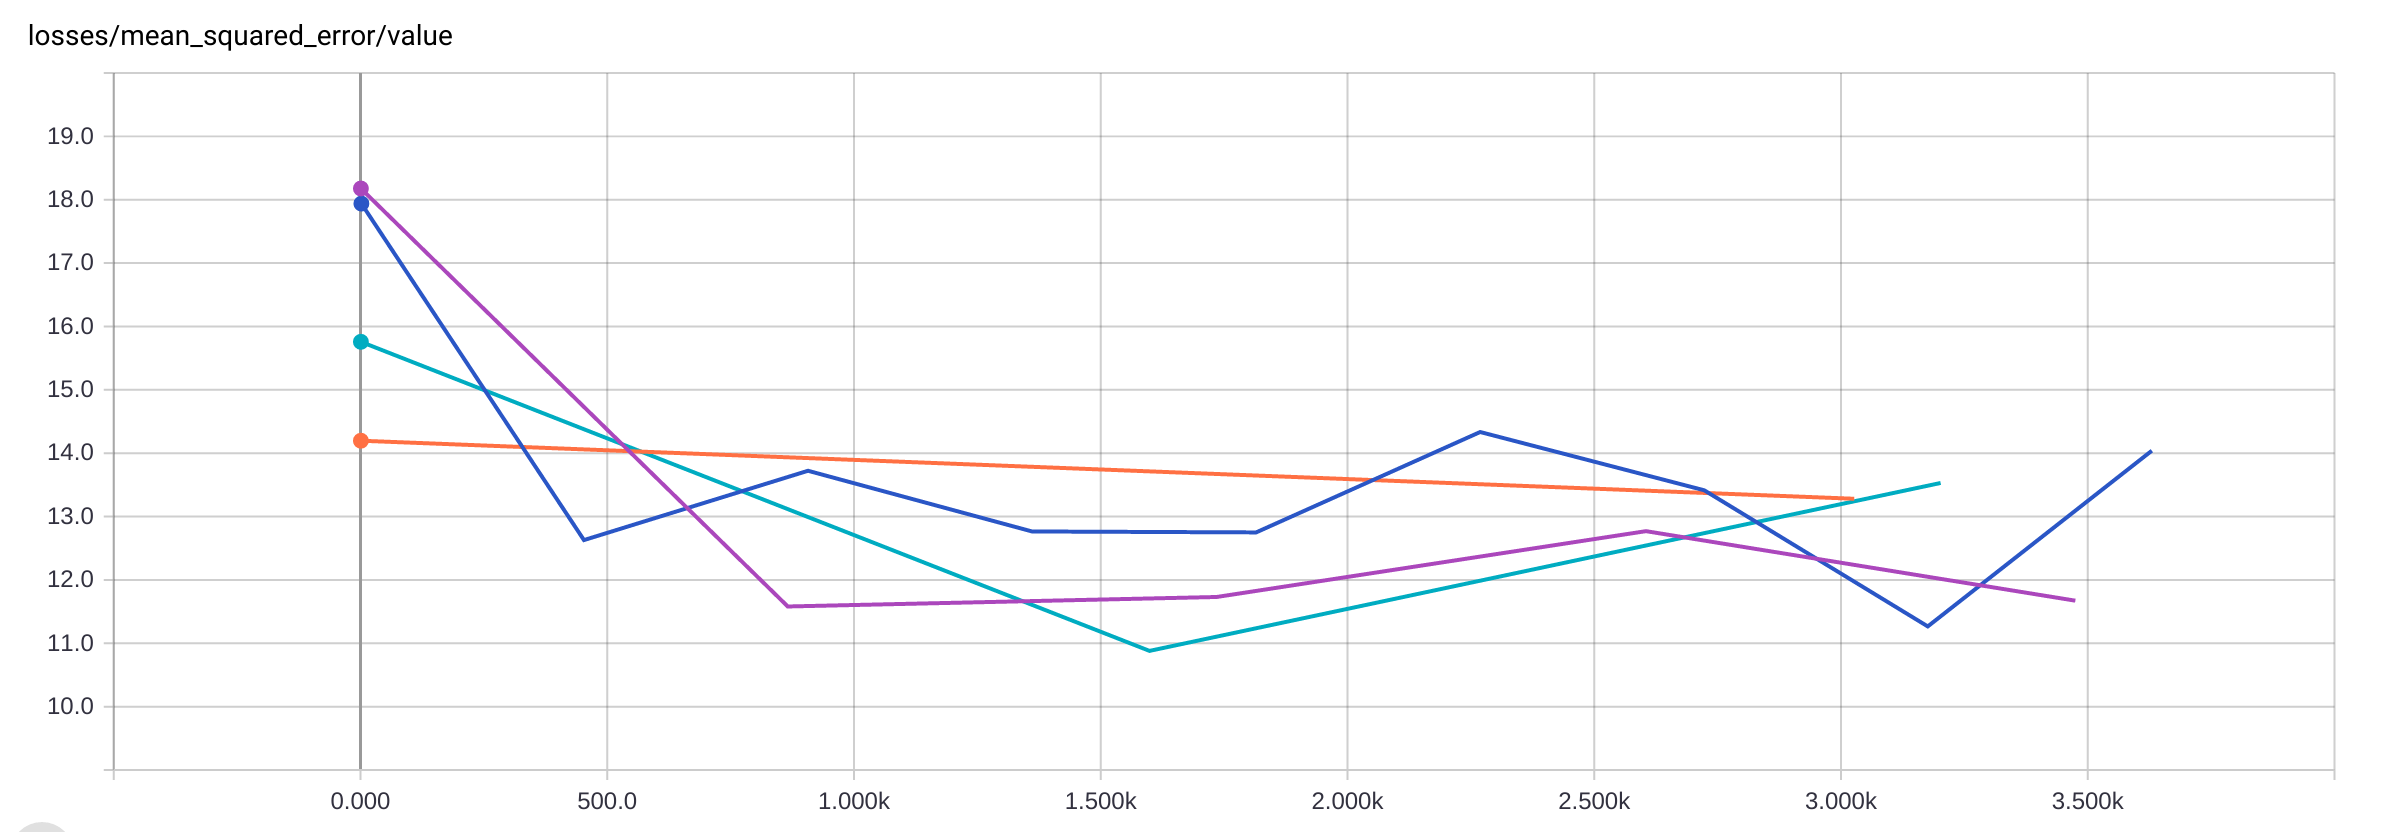
\includegraphics[width=1\textwidth]{figures/batch_size_valar_inception.png}
  \caption{Training loss against number of steps for different batch sizes:
  32=orange, 64=cyan, 128=magenta, 256=blue}
  \label{fig:batch_size_valar_inception}
\end{figure}


\subsubsection{Evaluation}

To evaluate our model, we use the independent test set of 200 images and we
report the mean squared error and the root mean squared error. For the
Inception V2 network defined above, with the selected batch size of 128 and
1,500 steps, we get the following measures:

\begin{align}
  MSE &= 15.655972 \\
  RMSE &= 3.9567628
\end{align}

However, these are not the best results that we have found. Indeed, it turns
out that using the VGG 16 model with a batch size of 32 and an initial learning
rate of 0.01 (keeping all other hyper-parameters the same as in section
\ref{sec:valar_fine}), we find the following measures:

\begin{align}
  MSE &= 13.749833 \\
  RMSE &= 3.7080767
\end{align}


\clearpage
\section{Future Work}


\subsection{Valence and Arousal Regression}

\subsubsection{Larger Dataset}

The small size of the data set (1,000 images) used to train the networks in
sections (\ref{sec:valar_inception_v2}) does not
allow for an effective training of deep learning models as these thrive on
large data sets. 

As such, one way to cheaply increase the number of images would be to perform
some data augmentation. The following operations could be applied to each image
in order to multiply the size of the data set by at least a factor of 4:

\begin{enumerate}
  \item flip image upside down or left to right
  \item rotate with a uniform random angle between 0 and 360 degrees
  \item random crop
  \item colour perturbation
\end{enumerate}


However, this does not replace the fact that the remaining images in the
data set should also be annotated manually for valence and arousal. Since we
are at the beginning of using machine learning to predict valence and arousal,
this first manual annotation is necessary if we wish to train a model that
could then replace/accelerate human annotators.

\subsubsection{More Models and Full Training}

It would be worth trying out more models on this data set, especially the
newer versions of the Inception model (versions 3 and 4). Furthermore, building
a custom model could be worthwhile, although one would probably have to
pre-train it on other available data sets for better results which could be
time consuming and computationally expensive. 

Furthermore, we do not train the Inception V2 or VGG 16 models from scratch in
this project and it would be interesting to see if performing training from
scratch is more beneficial in terms of model performance. Instead of training
from scratch, one could also fine-tune the whole model, not just the fully
connected layers. That is, we start with pre-existing weights which are all set
to be trainable in order to fine-tune them by using a small initial learning
rate, say $\alpha=0.001$.

\subsection{Video Analysis}

So far, we have only considered images. However, being able to continuously
predict valence and arousal on video data would be extremely useful. Training a
Deep Convolutional Neural Network on temporal sequences is an area of intense
research as being able to interpret emotions from videos has multiple
applications, including Human Computer Interaction.

\subsubsection{Recurrent Neural Networks}

One type model that could be used for video analysis is a Deep Convolutional
Network with a recurrent neural net instead of fully connected layers after the
convolutional layers. One type of recurrent network in particular is the Long
Short Term Memory, or LSTM, network which is accepted as the best recurrent
network for classification/regression of time series (Google uses LSTMs in
their speech recognition software).

\subsubsection{3D Convolutional Network}

Another type of model that could be used for video analysis is a 3D
convolutional neural network \cite{RefWorks:6} in which convolutions are extended to the
temporal dimension as well (see Fig.~\ref{fig:3d_conv})

\begin{figure}[ht]
  \centering
  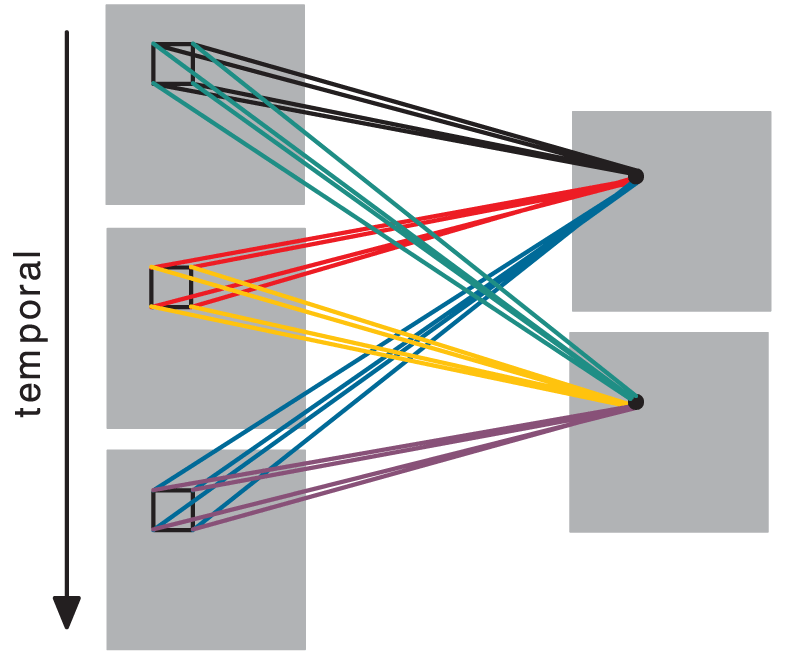
\includegraphics[scale=0.25]{figures/3d_conv.png}
  \caption{Example of a 3D convolution, note that connections with the same
  colours share the same weights}
  \source{\cite{RefWorks:6}}
  \label{fig:3d_conv}
\end{figure}

% REFERENCES
\clearpage
\bibliographystyle{plain}
\bibliography{refs.bib}

\appendix


\end{document}
%%% Local Variables: 
%%% mode: latex
%%% TeX-master: t
%%% End: 
